\chapter{Generative Neural Networks}\label{chap:Arch1}

This chapter introduces the notion of a convolutional neural network and its components, then goes over the specific network architectures we have worked with to solve the denoising problem. All networks presented is this chapter are generative, that is they take an image of $W\times H$ pixels with three channels and generate a new image of the same dimensions. Generative networks differ from other network types of convolutional neural networks which have different output shapes, such as classification networks which output one to a few nodes each indicating the probability that an object is present, and segmentation networks which usually have the same shape as the input but one output channel per segmented feature.

\section{Convolutional neural networks}
%- Introduce convolutional neural networks

We use deep convolutional neural networks which are neural networks based on the multilayer perceptron; that is, input data from one layer is sent to the neurons of the next layer and a dot product is performed between that input data and the next layer's learned weights. This process goes on for each layer. The main difference between a multilayer perceptrons and a \ac{CNN} is that a \ac{CNN} is not fully connected (that is neurons in one layer only receive a subset of the previous layer's neurons), instead, a \ac{CNN} takes advantage of the local spatial coherence of the input images to share weights and thus reduce the number of shared parameters.

The first and last layer have the same shape as the input image, that is its height, width, and 3-channels representing the RGB color-space. Most layers are hidden layers between the first and last one and contain many more channels (also called feature maps). Hidden layers are usually convolution (or transposed convolution) layers, activation layers, or pooling layers.

A loss function is applied to the output of the last layer, its gradient with respect to the network's weights is calculated with the backpropagation algorithm, and the Adam gradient-descent algorithm\cite{adam} adjusts the weights at the end of each batch training iteration. The learning rate needs to be fine-tuned to optimize fast learning without over-fitting.

\subsection{Layers}

\begin{figure}
  \begin{center}
    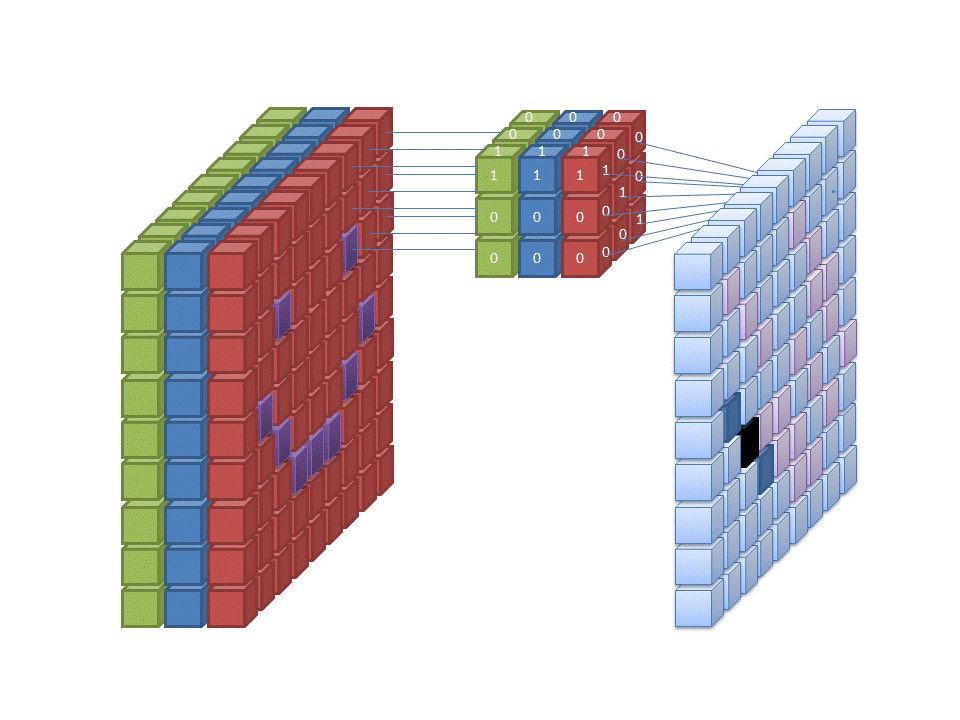
\includegraphics{gfx/Convolutional_Neural_Network_with_Color_Image_Filter.png}
    \caption[Standard convolution]{A filter is applied to the first 3-channels (RGB) input of an image in a convolutional neural network. The same filter is applied across all channels of the whole image as shown, and many of these filters are applied to form the following layer's feature map (I.e. its channels). Illustration by Wikimedia Commons user Cecbur (CC-BY-SA-4.0 license)}
    \label{fig:convolutionfilter}
  \end{center}
\end{figure}

\textbf{Convolution layers} apply convolutions with $C$ filters (also called features) to every $\acs{k}*\acs{k}$ area in the previous layer's width and height\footnote{assuming a stride of 1}, taking in every channel and returning one value per filter. Convolutions have a receptive field that is determined by kernel size \acs{k} (typical values for $\acs{k}$ are 3 and 5). The next layer's width and height is thus reduced unless padding is applied. Given an input layer's width or height dimension $d$ and \ac{p}, a convolution layer's output size can be calculated as $d-\ac{k}+2\ac{p}+1$. Each filter is weighted and weights are learned parameters. The same stack of filters is applied on every $\ac{k}*\ac{k}$ area of a given layer, therefore \acs{CNN} have largely reduced number of weight parameters.

\textbf{Activation layers} introduce non-linearity; they apply an activation function to every value in the previous layer and the resulting layer has the same shape as its input layer. We use the Sigmoid ($\phi(z)={1\over{1+e^{-z}}}$) and \ac{ReLU} ($R(z)=\max(0,z)$) activation functions. 

% add gradient descent, BN

\subsection{Loss function}
% therefore and however are not interchangeable but they are used the same way with the punctuation sort of like that yeah they should never have as pace on either side words
The loss function assigns a score to the generated images with respect to the provided ground-truth. A loss function should not simply compare the difference between generated and ground-truth pixels because there is no one-to-one mapping between clean and noisy images. Therefore, a loss function which only focuses on the difference between pixels favors denoised images whose pixels average the many acceptable values; i.e. the network is trained to generate blurry images. \cite{pix2pix}

The \ac{MSE} (or $\ell 2$) measures the average squared difference between the generated and ground-truth pixels, it is a simple yet effective loss function. Similarly the $\ell 1$ loss measures the sum of the absolute differences between ground-truth and generated pixels, this typically favors blurrier results. The \ac{SSIM} index is another metric which puts weights on structural information that is more likely to be perceived in images, namely local changes in luminance, contrast, and structure. A loss may also be learned such as the discriminator in a \ac{GAN}.

%https://arxiv.org/pdf/1511.08861.pdf
Mixing different losses often appears to yield better results \cite{lossescomp}, although it is sometimes challenging to combine them because they are often scaled differently (and training may suffer a performance penalty when having to compute multiple losses). Another valid approach is to switch loss function once convergence has been attained with one. \cite{lossescomp} We typically use the \ac{SSIM} index in our standard models and a combination of loss functions in the more challenging \ac{GAN}.

\marginpar{TODO: batch normalization}

\section{Network architectures}
\subsection{DnCNN}
DnCNN is a simple flat architecture \ac{CNN} architecture introduced in \cite{dncnn} to denoise images with residual learning. The network performs end-to-end denoising using only a convolution layer followed by \ac{BN} and a \ac{ReLU} activation layer at each depth level. The dimensions of the layers remain constant because the convolutions are padded appropriately ($\ac{p}={\ac{k}-1\over{2}}$). %The authors used a depth of 20 for blind gaussian denoising and set $\ac{k}=3$

The main contribution introduced in \cite{dncnn} appears to be the use of residual learning to speed up learning by modeling and subtracting the residual noise rather than generating a clean image. The use of a simple DnCNN architecture may have been introduced to emphasize the effectiveness of residual learning. DnCNN is the first network we experimented with, and although most of our experiment focus on the subsequent networks, we tested the author's residual learning theory with our dataset of ISO noise and all three networks.
\subsection{RED-Net}
The \ac{RED-Net} architecture is a residual encoder-decoder network. The first half of the network encodes the image using convolutions without padding such that the layers' dimensions continuously decrease, then the second half of the network (decoder) is made of transposed convolution layers that increase the layers' dimensions up to the original image's height and width. A \ac{ReLU} activation layer is placed between every (de)convolution layer. What is referred to as a residual network differs from the residual learning of \cite{dncnn}, a residual network has skip connections which in the case of \cite{rednet} are placed every two convolution layers and connect them to transposed convolution layers of matching dimensions. These skip connections add details that may have been lost in the encoding process to the output of the transposed convolutions. 
\subsection{U-Net}
The U-Net architecture is an encoder-decoder with skip connections originally designed for image segmentation. Its use in an image generator is possible by using the number of input color channels as output features and upsampling the resulting image. Each U-Net block applies two 3x3 convolutions followed by a parameter-free pooling operation that downsamples the image by a factor of two. The first block has 64 filters and the number of filters doubles after every pooling operation until there are 1024 filters. From this point the downsampling pooling operations are replaced with 2x2 upsampling transposed convolutions and the number of filters get halved every time, but the convolutions remain (as opposed to using transposed convolutions) so the layers' size remain smaller on the upsampling stage than it is originally. (This design results in corrupted borders which need to be discarded.) The U-Net architecture uses significantly less resources than conventional encoder-decoder networks and it is able to capture details at multiple frequencies.
\subsection{HulbNet}
We designed a multi-scale architecture somewhat similar to U-Net whose aim is to be more adapted to the denoising problem at hand. HulbNet uses the following concepts:
\begin{figure}
  \begin{center}
    \animategraphics[width=\textwidth/3*2]{1}{gfx/dilation/frame-}{0}{8}
    \caption[Dilated convolution]{Dilated convolution (dilation=2). Illustration by GitHub user vdumoulin (MIT license)}
    \label{fig:dilated}
  \end{center}
\end{figure}
\begin{figure}
  \begin{center}
  % Graphic for TeX using PGF
% Title: /orb/Dev/mthesis-denoise/thesis/gfx/convstr3.dia
% Creator: Dia v0.97.3
% CreationDate: Sun May 19 19:55:18 2019
% For: trougnouf
% \usepackage{tikz}
% The following commands are not supported in PSTricks at present
% We define them conditionally, so when they are implemented,
% this pgf file will use them.
\ifx\du\undefined
  \newlength{\du}
\fi
\setlength{\du}{15\unitlength}
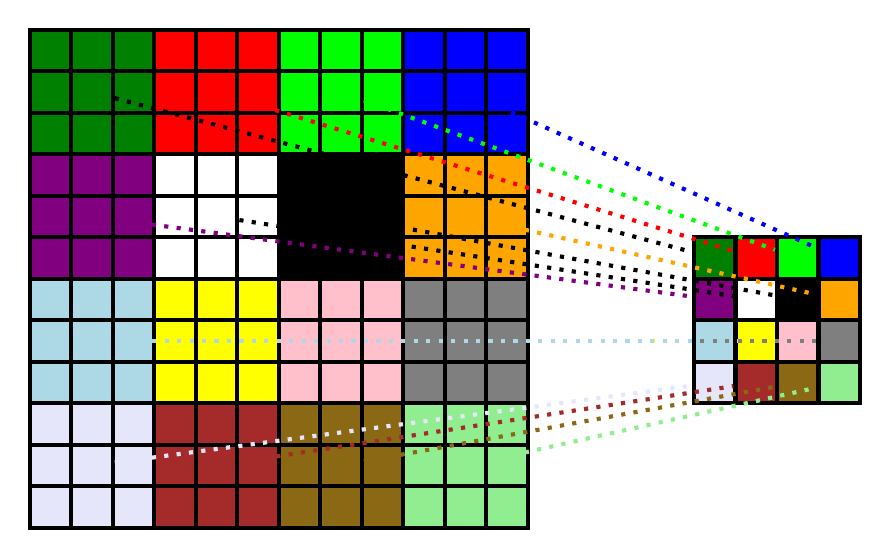
\begin{tikzpicture}
\pgftransformxscale{1.000000}
\pgftransformyscale{-1.000000}
\definecolor{dialinecolor}{rgb}{0.000000, 0.000000, 0.000000}
\pgfsetstrokecolor{dialinecolor}
\definecolor{dialinecolor}{rgb}{1.000000, 1.000000, 1.000000}
\pgfsetfillcolor{dialinecolor}
\pgfsetlinewidth{0.100000\du}
\pgfsetdash{}{0pt}
\pgfsetdash{}{0pt}
\pgfsetmiterjoin
\definecolor{dialinecolor}{rgb}{0.000000, 0.501961, 0.000000}
\pgfsetfillcolor{dialinecolor}
\fill (28.000000\du,10.000000\du)--(28.000000\du,11.000000\du)--(29.000000\du,11.000000\du)--(29.000000\du,10.000000\du)--cycle;
\definecolor{dialinecolor}{rgb}{0.000000, 0.000000, 0.000000}
\pgfsetstrokecolor{dialinecolor}
\draw (28.000000\du,10.000000\du)--(28.000000\du,11.000000\du)--(29.000000\du,11.000000\du)--(29.000000\du,10.000000\du)--cycle;
\pgfsetlinewidth{0.100000\du}
\pgfsetdash{}{0pt}
\pgfsetdash{}{0pt}
\pgfsetmiterjoin
\definecolor{dialinecolor}{rgb}{0.501961, 0.000000, 0.501961}
\pgfsetfillcolor{dialinecolor}
\fill (28.000000\du,11.000000\du)--(28.000000\du,12.000000\du)--(29.000000\du,12.000000\du)--(29.000000\du,11.000000\du)--cycle;
\definecolor{dialinecolor}{rgb}{0.000000, 0.000000, 0.000000}
\pgfsetstrokecolor{dialinecolor}
\draw (28.000000\du,11.000000\du)--(28.000000\du,12.000000\du)--(29.000000\du,12.000000\du)--(29.000000\du,11.000000\du)--cycle;
\pgfsetlinewidth{0.100000\du}
\pgfsetdash{}{0pt}
\pgfsetdash{}{0pt}
\pgfsetmiterjoin
\definecolor{dialinecolor}{rgb}{0.678431, 0.847059, 0.901961}
\pgfsetfillcolor{dialinecolor}
\fill (28.000000\du,12.000000\du)--(28.000000\du,13.000000\du)--(29.000000\du,13.000000\du)--(29.000000\du,12.000000\du)--cycle;
\definecolor{dialinecolor}{rgb}{0.000000, 0.000000, 0.000000}
\pgfsetstrokecolor{dialinecolor}
\draw (28.000000\du,12.000000\du)--(28.000000\du,13.000000\du)--(29.000000\du,13.000000\du)--(29.000000\du,12.000000\du)--cycle;
\pgfsetlinewidth{0.100000\du}
\pgfsetdash{}{0pt}
\pgfsetdash{}{0pt}
\pgfsetmiterjoin
\definecolor{dialinecolor}{rgb}{0.901961, 0.901961, 0.980392}
\pgfsetfillcolor{dialinecolor}
\fill (28.000000\du,13.000000\du)--(28.000000\du,14.000000\du)--(29.000000\du,14.000000\du)--(29.000000\du,13.000000\du)--cycle;
\definecolor{dialinecolor}{rgb}{0.000000, 0.000000, 0.000000}
\pgfsetstrokecolor{dialinecolor}
\draw (28.000000\du,13.000000\du)--(28.000000\du,14.000000\du)--(29.000000\du,14.000000\du)--(29.000000\du,13.000000\du)--cycle;
\pgfsetlinewidth{0.100000\du}
\pgfsetdash{}{0pt}
\pgfsetdash{}{0pt}
\pgfsetmiterjoin
\definecolor{dialinecolor}{rgb}{0.647059, 0.164706, 0.164706}
\pgfsetfillcolor{dialinecolor}
\fill (29.000000\du,13.000000\du)--(29.000000\du,14.000000\du)--(30.000000\du,14.000000\du)--(30.000000\du,13.000000\du)--cycle;
\definecolor{dialinecolor}{rgb}{0.000000, 0.000000, 0.000000}
\pgfsetstrokecolor{dialinecolor}
\draw (29.000000\du,13.000000\du)--(29.000000\du,14.000000\du)--(30.000000\du,14.000000\du)--(30.000000\du,13.000000\du)--cycle;
\pgfsetlinewidth{0.100000\du}
\pgfsetdash{}{0pt}
\pgfsetdash{}{0pt}
\pgfsetmiterjoin
\definecolor{dialinecolor}{rgb}{0.545098, 0.411765, 0.078431}
\pgfsetfillcolor{dialinecolor}
\fill (30.000000\du,13.000000\du)--(30.000000\du,14.000000\du)--(31.000000\du,14.000000\du)--(31.000000\du,13.000000\du)--cycle;
\definecolor{dialinecolor}{rgb}{0.000000, 0.000000, 0.000000}
\pgfsetstrokecolor{dialinecolor}
\draw (30.000000\du,13.000000\du)--(30.000000\du,14.000000\du)--(31.000000\du,14.000000\du)--(31.000000\du,13.000000\du)--cycle;
\pgfsetlinewidth{0.100000\du}
\pgfsetdash{}{0pt}
\pgfsetdash{}{0pt}
\pgfsetmiterjoin
\definecolor{dialinecolor}{rgb}{0.564706, 0.933333, 0.564706}
\pgfsetfillcolor{dialinecolor}
\fill (31.000000\du,13.000000\du)--(31.000000\du,14.000000\du)--(32.000000\du,14.000000\du)--(32.000000\du,13.000000\du)--cycle;
\definecolor{dialinecolor}{rgb}{0.000000, 0.000000, 0.000000}
\pgfsetstrokecolor{dialinecolor}
\draw (31.000000\du,13.000000\du)--(31.000000\du,14.000000\du)--(32.000000\du,14.000000\du)--(32.000000\du,13.000000\du)--cycle;
\pgfsetlinewidth{0.100000\du}
\pgfsetdash{}{0pt}
\pgfsetdash{}{0pt}
\pgfsetmiterjoin
\definecolor{dialinecolor}{rgb}{1.000000, 0.000000, 0.000000}
\pgfsetfillcolor{dialinecolor}
\fill (15.000000\du,5.000000\du)--(15.000000\du,6.000000\du)--(16.000000\du,6.000000\du)--(16.000000\du,5.000000\du)--cycle;
\definecolor{dialinecolor}{rgb}{0.000000, 0.000000, 0.000000}
\pgfsetstrokecolor{dialinecolor}
\draw (15.000000\du,5.000000\du)--(15.000000\du,6.000000\du)--(16.000000\du,6.000000\du)--(16.000000\du,5.000000\du)--cycle;
\pgfsetlinewidth{0.100000\du}
\pgfsetdash{}{0pt}
\pgfsetdash{}{0pt}
\pgfsetmiterjoin
\definecolor{dialinecolor}{rgb}{1.000000, 0.000000, 0.000000}
\pgfsetfillcolor{dialinecolor}
\fill (16.000000\du,5.000000\du)--(16.000000\du,6.000000\du)--(17.000000\du,6.000000\du)--(17.000000\du,5.000000\du)--cycle;
\definecolor{dialinecolor}{rgb}{0.000000, 0.000000, 0.000000}
\pgfsetstrokecolor{dialinecolor}
\draw (16.000000\du,5.000000\du)--(16.000000\du,6.000000\du)--(17.000000\du,6.000000\du)--(17.000000\du,5.000000\du)--cycle;
\pgfsetlinewidth{0.100000\du}
\pgfsetdash{}{0pt}
\pgfsetdash{}{0pt}
\pgfsetmiterjoin
\definecolor{dialinecolor}{rgb}{1.000000, 0.000000, 0.000000}
\pgfsetfillcolor{dialinecolor}
\fill (17.000000\du,5.000000\du)--(17.000000\du,6.000000\du)--(18.000000\du,6.000000\du)--(18.000000\du,5.000000\du)--cycle;
\definecolor{dialinecolor}{rgb}{0.000000, 0.000000, 0.000000}
\pgfsetstrokecolor{dialinecolor}
\draw (17.000000\du,5.000000\du)--(17.000000\du,6.000000\du)--(18.000000\du,6.000000\du)--(18.000000\du,5.000000\du)--cycle;
\pgfsetlinewidth{0.100000\du}
\pgfsetdash{}{0pt}
\pgfsetdash{}{0pt}
\pgfsetmiterjoin
\definecolor{dialinecolor}{rgb}{0.000000, 1.000000, 0.000000}
\pgfsetfillcolor{dialinecolor}
\fill (18.000000\du,5.000000\du)--(18.000000\du,6.000000\du)--(19.000000\du,6.000000\du)--(19.000000\du,5.000000\du)--cycle;
\definecolor{dialinecolor}{rgb}{0.000000, 0.000000, 0.000000}
\pgfsetstrokecolor{dialinecolor}
\draw (18.000000\du,5.000000\du)--(18.000000\du,6.000000\du)--(19.000000\du,6.000000\du)--(19.000000\du,5.000000\du)--cycle;
\pgfsetlinewidth{0.100000\du}
\pgfsetdash{}{0pt}
\pgfsetdash{}{0pt}
\pgfsetmiterjoin
\definecolor{dialinecolor}{rgb}{0.000000, 1.000000, 0.000000}
\pgfsetfillcolor{dialinecolor}
\fill (19.000000\du,5.000000\du)--(19.000000\du,6.000000\du)--(20.000000\du,6.000000\du)--(20.000000\du,5.000000\du)--cycle;
\definecolor{dialinecolor}{rgb}{0.000000, 0.000000, 0.000000}
\pgfsetstrokecolor{dialinecolor}
\draw (19.000000\du,5.000000\du)--(19.000000\du,6.000000\du)--(20.000000\du,6.000000\du)--(20.000000\du,5.000000\du)--cycle;
\pgfsetlinewidth{0.100000\du}
\pgfsetdash{}{0pt}
\pgfsetdash{}{0pt}
\pgfsetmiterjoin
\definecolor{dialinecolor}{rgb}{0.000000, 1.000000, 0.000000}
\pgfsetfillcolor{dialinecolor}
\fill (20.000000\du,5.000000\du)--(20.000000\du,6.000000\du)--(21.000000\du,6.000000\du)--(21.000000\du,5.000000\du)--cycle;
\definecolor{dialinecolor}{rgb}{0.000000, 0.000000, 0.000000}
\pgfsetstrokecolor{dialinecolor}
\draw (20.000000\du,5.000000\du)--(20.000000\du,6.000000\du)--(21.000000\du,6.000000\du)--(21.000000\du,5.000000\du)--cycle;
\pgfsetlinewidth{0.100000\du}
\pgfsetdash{}{0pt}
\pgfsetdash{}{0pt}
\pgfsetmiterjoin
\definecolor{dialinecolor}{rgb}{0.000000, 0.000000, 1.000000}
\pgfsetfillcolor{dialinecolor}
\fill (21.000000\du,5.000000\du)--(21.000000\du,6.000000\du)--(22.000000\du,6.000000\du)--(22.000000\du,5.000000\du)--cycle;
\definecolor{dialinecolor}{rgb}{0.000000, 0.000000, 0.000000}
\pgfsetstrokecolor{dialinecolor}
\draw (21.000000\du,5.000000\du)--(21.000000\du,6.000000\du)--(22.000000\du,6.000000\du)--(22.000000\du,5.000000\du)--cycle;
\pgfsetlinewidth{0.100000\du}
\pgfsetdash{}{0pt}
\pgfsetdash{}{0pt}
\pgfsetmiterjoin
\definecolor{dialinecolor}{rgb}{0.000000, 0.000000, 1.000000}
\pgfsetfillcolor{dialinecolor}
\fill (22.000000\du,5.000000\du)--(22.000000\du,6.000000\du)--(23.000000\du,6.000000\du)--(23.000000\du,5.000000\du)--cycle;
\definecolor{dialinecolor}{rgb}{0.000000, 0.000000, 0.000000}
\pgfsetstrokecolor{dialinecolor}
\draw (22.000000\du,5.000000\du)--(22.000000\du,6.000000\du)--(23.000000\du,6.000000\du)--(23.000000\du,5.000000\du)--cycle;
\pgfsetlinewidth{0.100000\du}
\pgfsetdash{}{0pt}
\pgfsetdash{}{0pt}
\pgfsetmiterjoin
\definecolor{dialinecolor}{rgb}{0.000000, 0.000000, 1.000000}
\pgfsetfillcolor{dialinecolor}
\fill (23.000000\du,5.000000\du)--(23.000000\du,6.000000\du)--(24.000000\du,6.000000\du)--(24.000000\du,5.000000\du)--cycle;
\definecolor{dialinecolor}{rgb}{0.000000, 0.000000, 0.000000}
\pgfsetstrokecolor{dialinecolor}
\draw (23.000000\du,5.000000\du)--(23.000000\du,6.000000\du)--(24.000000\du,6.000000\du)--(24.000000\du,5.000000\du)--cycle;
\pgfsetlinewidth{0.100000\du}
\pgfsetdash{}{0pt}
\pgfsetdash{}{0pt}
\pgfsetmiterjoin
\definecolor{dialinecolor}{rgb}{1.000000, 0.000000, 0.000000}
\pgfsetfillcolor{dialinecolor}
\fill (15.000000\du,6.000000\du)--(15.000000\du,7.000000\du)--(16.000000\du,7.000000\du)--(16.000000\du,6.000000\du)--cycle;
\definecolor{dialinecolor}{rgb}{0.000000, 0.000000, 0.000000}
\pgfsetstrokecolor{dialinecolor}
\draw (15.000000\du,6.000000\du)--(15.000000\du,7.000000\du)--(16.000000\du,7.000000\du)--(16.000000\du,6.000000\du)--cycle;
\pgfsetlinewidth{0.100000\du}
\pgfsetdash{}{0pt}
\pgfsetdash{}{0pt}
\pgfsetmiterjoin
\definecolor{dialinecolor}{rgb}{1.000000, 0.000000, 0.000000}
\pgfsetfillcolor{dialinecolor}
\fill (16.000000\du,6.000000\du)--(16.000000\du,7.000000\du)--(17.000000\du,7.000000\du)--(17.000000\du,6.000000\du)--cycle;
\definecolor{dialinecolor}{rgb}{0.000000, 0.000000, 0.000000}
\pgfsetstrokecolor{dialinecolor}
\draw (16.000000\du,6.000000\du)--(16.000000\du,7.000000\du)--(17.000000\du,7.000000\du)--(17.000000\du,6.000000\du)--cycle;
\pgfsetlinewidth{0.100000\du}
\pgfsetdash{}{0pt}
\pgfsetdash{}{0pt}
\pgfsetmiterjoin
\definecolor{dialinecolor}{rgb}{1.000000, 0.000000, 0.000000}
\pgfsetfillcolor{dialinecolor}
\fill (17.000000\du,6.000000\du)--(17.000000\du,7.000000\du)--(18.000000\du,7.000000\du)--(18.000000\du,6.000000\du)--cycle;
\definecolor{dialinecolor}{rgb}{0.000000, 0.000000, 0.000000}
\pgfsetstrokecolor{dialinecolor}
\draw (17.000000\du,6.000000\du)--(17.000000\du,7.000000\du)--(18.000000\du,7.000000\du)--(18.000000\du,6.000000\du)--cycle;
\pgfsetlinewidth{0.100000\du}
\pgfsetdash{}{0pt}
\pgfsetdash{}{0pt}
\pgfsetmiterjoin
\definecolor{dialinecolor}{rgb}{0.000000, 1.000000, 0.000000}
\pgfsetfillcolor{dialinecolor}
\fill (18.000000\du,6.000000\du)--(18.000000\du,7.000000\du)--(19.000000\du,7.000000\du)--(19.000000\du,6.000000\du)--cycle;
\definecolor{dialinecolor}{rgb}{0.000000, 0.000000, 0.000000}
\pgfsetstrokecolor{dialinecolor}
\draw (18.000000\du,6.000000\du)--(18.000000\du,7.000000\du)--(19.000000\du,7.000000\du)--(19.000000\du,6.000000\du)--cycle;
\pgfsetlinewidth{0.100000\du}
\pgfsetdash{}{0pt}
\pgfsetdash{}{0pt}
\pgfsetmiterjoin
\definecolor{dialinecolor}{rgb}{0.000000, 1.000000, 0.000000}
\pgfsetfillcolor{dialinecolor}
\fill (19.000000\du,6.000000\du)--(19.000000\du,7.000000\du)--(20.000000\du,7.000000\du)--(20.000000\du,6.000000\du)--cycle;
\definecolor{dialinecolor}{rgb}{0.000000, 0.000000, 0.000000}
\pgfsetstrokecolor{dialinecolor}
\draw (19.000000\du,6.000000\du)--(19.000000\du,7.000000\du)--(20.000000\du,7.000000\du)--(20.000000\du,6.000000\du)--cycle;
\pgfsetlinewidth{0.100000\du}
\pgfsetdash{}{0pt}
\pgfsetdash{}{0pt}
\pgfsetmiterjoin
\definecolor{dialinecolor}{rgb}{0.000000, 1.000000, 0.000000}
\pgfsetfillcolor{dialinecolor}
\fill (20.000000\du,6.000000\du)--(20.000000\du,7.000000\du)--(21.000000\du,7.000000\du)--(21.000000\du,6.000000\du)--cycle;
\definecolor{dialinecolor}{rgb}{0.000000, 0.000000, 0.000000}
\pgfsetstrokecolor{dialinecolor}
\draw (20.000000\du,6.000000\du)--(20.000000\du,7.000000\du)--(21.000000\du,7.000000\du)--(21.000000\du,6.000000\du)--cycle;
\pgfsetlinewidth{0.100000\du}
\pgfsetdash{}{0pt}
\pgfsetdash{}{0pt}
\pgfsetmiterjoin
\definecolor{dialinecolor}{rgb}{0.000000, 0.000000, 1.000000}
\pgfsetfillcolor{dialinecolor}
\fill (21.000000\du,6.000000\du)--(21.000000\du,7.000000\du)--(22.000000\du,7.000000\du)--(22.000000\du,6.000000\du)--cycle;
\definecolor{dialinecolor}{rgb}{0.000000, 0.000000, 0.000000}
\pgfsetstrokecolor{dialinecolor}
\draw (21.000000\du,6.000000\du)--(21.000000\du,7.000000\du)--(22.000000\du,7.000000\du)--(22.000000\du,6.000000\du)--cycle;
\pgfsetlinewidth{0.100000\du}
\pgfsetdash{}{0pt}
\pgfsetdash{}{0pt}
\pgfsetmiterjoin
\definecolor{dialinecolor}{rgb}{0.000000, 0.000000, 1.000000}
\pgfsetfillcolor{dialinecolor}
\fill (22.000000\du,6.000000\du)--(22.000000\du,7.000000\du)--(23.000000\du,7.000000\du)--(23.000000\du,6.000000\du)--cycle;
\definecolor{dialinecolor}{rgb}{0.000000, 0.000000, 0.000000}
\pgfsetstrokecolor{dialinecolor}
\draw (22.000000\du,6.000000\du)--(22.000000\du,7.000000\du)--(23.000000\du,7.000000\du)--(23.000000\du,6.000000\du)--cycle;
\pgfsetlinewidth{0.100000\du}
\pgfsetdash{}{0pt}
\pgfsetdash{}{0pt}
\pgfsetmiterjoin
\definecolor{dialinecolor}{rgb}{0.000000, 0.000000, 1.000000}
\pgfsetfillcolor{dialinecolor}
\fill (23.000000\du,6.000000\du)--(23.000000\du,7.000000\du)--(24.000000\du,7.000000\du)--(24.000000\du,6.000000\du)--cycle;
\definecolor{dialinecolor}{rgb}{0.000000, 0.000000, 0.000000}
\pgfsetstrokecolor{dialinecolor}
\draw (23.000000\du,6.000000\du)--(23.000000\du,7.000000\du)--(24.000000\du,7.000000\du)--(24.000000\du,6.000000\du)--cycle;
\pgfsetlinewidth{0.100000\du}
\pgfsetdash{}{0pt}
\pgfsetdash{}{0pt}
\pgfsetmiterjoin
\definecolor{dialinecolor}{rgb}{1.000000, 0.000000, 0.000000}
\pgfsetfillcolor{dialinecolor}
\fill (15.000000\du,7.000000\du)--(15.000000\du,8.000000\du)--(16.000000\du,8.000000\du)--(16.000000\du,7.000000\du)--cycle;
\definecolor{dialinecolor}{rgb}{0.000000, 0.000000, 0.000000}
\pgfsetstrokecolor{dialinecolor}
\draw (15.000000\du,7.000000\du)--(15.000000\du,8.000000\du)--(16.000000\du,8.000000\du)--(16.000000\du,7.000000\du)--cycle;
\pgfsetlinewidth{0.100000\du}
\pgfsetdash{}{0pt}
\pgfsetdash{}{0pt}
\pgfsetmiterjoin
\definecolor{dialinecolor}{rgb}{1.000000, 0.000000, 0.000000}
\pgfsetfillcolor{dialinecolor}
\fill (16.000000\du,7.000000\du)--(16.000000\du,8.000000\du)--(17.000000\du,8.000000\du)--(17.000000\du,7.000000\du)--cycle;
\definecolor{dialinecolor}{rgb}{0.000000, 0.000000, 0.000000}
\pgfsetstrokecolor{dialinecolor}
\draw (16.000000\du,7.000000\du)--(16.000000\du,8.000000\du)--(17.000000\du,8.000000\du)--(17.000000\du,7.000000\du)--cycle;
\pgfsetlinewidth{0.100000\du}
\pgfsetdash{}{0pt}
\pgfsetdash{}{0pt}
\pgfsetmiterjoin
\definecolor{dialinecolor}{rgb}{1.000000, 0.000000, 0.000000}
\pgfsetfillcolor{dialinecolor}
\fill (17.000000\du,7.000000\du)--(17.000000\du,8.000000\du)--(18.000000\du,8.000000\du)--(18.000000\du,7.000000\du)--cycle;
\definecolor{dialinecolor}{rgb}{0.000000, 0.000000, 0.000000}
\pgfsetstrokecolor{dialinecolor}
\draw (17.000000\du,7.000000\du)--(17.000000\du,8.000000\du)--(18.000000\du,8.000000\du)--(18.000000\du,7.000000\du)--cycle;
\pgfsetlinewidth{0.100000\du}
\pgfsetdash{}{0pt}
\pgfsetdash{}{0pt}
\pgfsetmiterjoin
\definecolor{dialinecolor}{rgb}{0.000000, 1.000000, 0.000000}
\pgfsetfillcolor{dialinecolor}
\fill (18.000000\du,7.000000\du)--(18.000000\du,8.000000\du)--(19.000000\du,8.000000\du)--(19.000000\du,7.000000\du)--cycle;
\definecolor{dialinecolor}{rgb}{0.000000, 0.000000, 0.000000}
\pgfsetstrokecolor{dialinecolor}
\draw (18.000000\du,7.000000\du)--(18.000000\du,8.000000\du)--(19.000000\du,8.000000\du)--(19.000000\du,7.000000\du)--cycle;
\pgfsetlinewidth{0.100000\du}
\pgfsetdash{}{0pt}
\pgfsetdash{}{0pt}
\pgfsetmiterjoin
\definecolor{dialinecolor}{rgb}{0.000000, 1.000000, 0.000000}
\pgfsetfillcolor{dialinecolor}
\fill (19.000000\du,7.000000\du)--(19.000000\du,8.000000\du)--(20.000000\du,8.000000\du)--(20.000000\du,7.000000\du)--cycle;
\definecolor{dialinecolor}{rgb}{0.000000, 0.000000, 0.000000}
\pgfsetstrokecolor{dialinecolor}
\draw (19.000000\du,7.000000\du)--(19.000000\du,8.000000\du)--(20.000000\du,8.000000\du)--(20.000000\du,7.000000\du)--cycle;
\pgfsetlinewidth{0.100000\du}
\pgfsetdash{}{0pt}
\pgfsetdash{}{0pt}
\pgfsetmiterjoin
\definecolor{dialinecolor}{rgb}{0.000000, 1.000000, 0.000000}
\pgfsetfillcolor{dialinecolor}
\fill (20.000000\du,7.000000\du)--(20.000000\du,8.000000\du)--(21.000000\du,8.000000\du)--(21.000000\du,7.000000\du)--cycle;
\definecolor{dialinecolor}{rgb}{0.000000, 0.000000, 0.000000}
\pgfsetstrokecolor{dialinecolor}
\draw (20.000000\du,7.000000\du)--(20.000000\du,8.000000\du)--(21.000000\du,8.000000\du)--(21.000000\du,7.000000\du)--cycle;
\pgfsetlinewidth{0.100000\du}
\pgfsetdash{}{0pt}
\pgfsetdash{}{0pt}
\pgfsetmiterjoin
\definecolor{dialinecolor}{rgb}{0.000000, 0.000000, 1.000000}
\pgfsetfillcolor{dialinecolor}
\fill (21.000000\du,7.000000\du)--(21.000000\du,8.000000\du)--(22.000000\du,8.000000\du)--(22.000000\du,7.000000\du)--cycle;
\definecolor{dialinecolor}{rgb}{0.000000, 0.000000, 0.000000}
\pgfsetstrokecolor{dialinecolor}
\draw (21.000000\du,7.000000\du)--(21.000000\du,8.000000\du)--(22.000000\du,8.000000\du)--(22.000000\du,7.000000\du)--cycle;
\pgfsetlinewidth{0.100000\du}
\pgfsetdash{}{0pt}
\pgfsetdash{}{0pt}
\pgfsetmiterjoin
\definecolor{dialinecolor}{rgb}{0.000000, 0.000000, 1.000000}
\pgfsetfillcolor{dialinecolor}
\fill (22.000000\du,7.000000\du)--(22.000000\du,8.000000\du)--(23.000000\du,8.000000\du)--(23.000000\du,7.000000\du)--cycle;
\definecolor{dialinecolor}{rgb}{0.000000, 0.000000, 0.000000}
\pgfsetstrokecolor{dialinecolor}
\draw (22.000000\du,7.000000\du)--(22.000000\du,8.000000\du)--(23.000000\du,8.000000\du)--(23.000000\du,7.000000\du)--cycle;
\pgfsetlinewidth{0.100000\du}
\pgfsetdash{}{0pt}
\pgfsetdash{}{0pt}
\pgfsetmiterjoin
\definecolor{dialinecolor}{rgb}{0.000000, 0.000000, 1.000000}
\pgfsetfillcolor{dialinecolor}
\fill (23.000000\du,7.000000\du)--(23.000000\du,8.000000\du)--(24.000000\du,8.000000\du)--(24.000000\du,7.000000\du)--cycle;
\definecolor{dialinecolor}{rgb}{0.000000, 0.000000, 0.000000}
\pgfsetstrokecolor{dialinecolor}
\draw (23.000000\du,7.000000\du)--(23.000000\du,8.000000\du)--(24.000000\du,8.000000\du)--(24.000000\du,7.000000\du)--cycle;
\pgfsetlinewidth{0.100000\du}
\pgfsetdash{}{0pt}
\pgfsetdash{}{0pt}
\pgfsetmiterjoin
\definecolor{dialinecolor}{rgb}{1.000000, 1.000000, 1.000000}
\pgfsetfillcolor{dialinecolor}
\fill (15.000000\du,8.000000\du)--(15.000000\du,9.000000\du)--(16.000000\du,9.000000\du)--(16.000000\du,8.000000\du)--cycle;
\definecolor{dialinecolor}{rgb}{0.000000, 0.000000, 0.000000}
\pgfsetstrokecolor{dialinecolor}
\draw (15.000000\du,8.000000\du)--(15.000000\du,9.000000\du)--(16.000000\du,9.000000\du)--(16.000000\du,8.000000\du)--cycle;
\pgfsetlinewidth{0.100000\du}
\pgfsetdash{}{0pt}
\pgfsetdash{}{0pt}
\pgfsetmiterjoin
\definecolor{dialinecolor}{rgb}{1.000000, 1.000000, 1.000000}
\pgfsetfillcolor{dialinecolor}
\fill (16.000000\du,8.000000\du)--(16.000000\du,9.000000\du)--(17.000000\du,9.000000\du)--(17.000000\du,8.000000\du)--cycle;
\definecolor{dialinecolor}{rgb}{0.000000, 0.000000, 0.000000}
\pgfsetstrokecolor{dialinecolor}
\draw (16.000000\du,8.000000\du)--(16.000000\du,9.000000\du)--(17.000000\du,9.000000\du)--(17.000000\du,8.000000\du)--cycle;
\pgfsetlinewidth{0.100000\du}
\pgfsetdash{}{0pt}
\pgfsetdash{}{0pt}
\pgfsetmiterjoin
\definecolor{dialinecolor}{rgb}{1.000000, 1.000000, 1.000000}
\pgfsetfillcolor{dialinecolor}
\fill (17.000000\du,8.000000\du)--(17.000000\du,9.000000\du)--(18.000000\du,9.000000\du)--(18.000000\du,8.000000\du)--cycle;
\definecolor{dialinecolor}{rgb}{0.000000, 0.000000, 0.000000}
\pgfsetstrokecolor{dialinecolor}
\draw (17.000000\du,8.000000\du)--(17.000000\du,9.000000\du)--(18.000000\du,9.000000\du)--(18.000000\du,8.000000\du)--cycle;
\pgfsetlinewidth{0.100000\du}
\pgfsetdash{}{0pt}
\pgfsetdash{}{0pt}
\pgfsetmiterjoin
\definecolor{dialinecolor}{rgb}{0.000000, 0.000000, 0.000000}
\pgfsetstrokecolor{dialinecolor}
\draw (18.000000\du,8.000000\du)--(18.000000\du,9.000000\du)--(19.000000\du,9.000000\du)--(19.000000\du,8.000000\du)--cycle;
\pgfsetlinewidth{0.100000\du}
\pgfsetdash{}{0pt}
\pgfsetdash{}{0pt}
\pgfsetmiterjoin
\definecolor{dialinecolor}{rgb}{0.000000, 0.000000, 0.000000}
\pgfsetfillcolor{dialinecolor}
\fill (18.000000\du,8.000000\du)--(18.000000\du,9.000000\du)--(19.000000\du,9.000000\du)--(19.000000\du,8.000000\du)--cycle;
\definecolor{dialinecolor}{rgb}{0.000000, 0.000000, 0.000000}
\pgfsetstrokecolor{dialinecolor}
\draw (18.000000\du,8.000000\du)--(18.000000\du,9.000000\du)--(19.000000\du,9.000000\du)--(19.000000\du,8.000000\du)--cycle;
\pgfsetlinewidth{0.100000\du}
\pgfsetdash{}{0pt}
\pgfsetdash{}{0pt}
\pgfsetmiterjoin
\definecolor{dialinecolor}{rgb}{0.000000, 0.000000, 0.000000}
\pgfsetfillcolor{dialinecolor}
\fill (20.000000\du,8.000000\du)--(20.000000\du,9.000000\du)--(21.000000\du,9.000000\du)--(21.000000\du,8.000000\du)--cycle;
\definecolor{dialinecolor}{rgb}{0.000000, 0.000000, 0.000000}
\pgfsetstrokecolor{dialinecolor}
\draw (20.000000\du,8.000000\du)--(20.000000\du,9.000000\du)--(21.000000\du,9.000000\du)--(21.000000\du,8.000000\du)--cycle;
\pgfsetlinewidth{0.100000\du}
\pgfsetdash{}{0pt}
\pgfsetdash{}{0pt}
\pgfsetmiterjoin
\definecolor{dialinecolor}{rgb}{1.000000, 0.647059, 0.000000}
\pgfsetfillcolor{dialinecolor}
\fill (21.000000\du,8.000000\du)--(21.000000\du,9.000000\du)--(22.000000\du,9.000000\du)--(22.000000\du,8.000000\du)--cycle;
\definecolor{dialinecolor}{rgb}{0.000000, 0.000000, 0.000000}
\pgfsetstrokecolor{dialinecolor}
\draw (21.000000\du,8.000000\du)--(21.000000\du,9.000000\du)--(22.000000\du,9.000000\du)--(22.000000\du,8.000000\du)--cycle;
\pgfsetlinewidth{0.100000\du}
\pgfsetdash{}{0pt}
\pgfsetdash{}{0pt}
\pgfsetmiterjoin
\definecolor{dialinecolor}{rgb}{1.000000, 0.647059, 0.000000}
\pgfsetfillcolor{dialinecolor}
\fill (22.000000\du,8.000000\du)--(22.000000\du,9.000000\du)--(23.000000\du,9.000000\du)--(23.000000\du,8.000000\du)--cycle;
\definecolor{dialinecolor}{rgb}{0.000000, 0.000000, 0.000000}
\pgfsetstrokecolor{dialinecolor}
\draw (22.000000\du,8.000000\du)--(22.000000\du,9.000000\du)--(23.000000\du,9.000000\du)--(23.000000\du,8.000000\du)--cycle;
\pgfsetlinewidth{0.100000\du}
\pgfsetdash{}{0pt}
\pgfsetdash{}{0pt}
\pgfsetmiterjoin
\definecolor{dialinecolor}{rgb}{1.000000, 0.647059, 0.000000}
\pgfsetfillcolor{dialinecolor}
\fill (23.000000\du,8.000000\du)--(23.000000\du,9.000000\du)--(24.000000\du,9.000000\du)--(24.000000\du,8.000000\du)--cycle;
\definecolor{dialinecolor}{rgb}{0.000000, 0.000000, 0.000000}
\pgfsetstrokecolor{dialinecolor}
\draw (23.000000\du,8.000000\du)--(23.000000\du,9.000000\du)--(24.000000\du,9.000000\du)--(24.000000\du,8.000000\du)--cycle;
\pgfsetlinewidth{0.100000\du}
\pgfsetdash{}{0pt}
\pgfsetdash{}{0pt}
\pgfsetmiterjoin
\definecolor{dialinecolor}{rgb}{1.000000, 1.000000, 1.000000}
\pgfsetfillcolor{dialinecolor}
\fill (15.000000\du,9.000000\du)--(15.000000\du,10.000000\du)--(16.000000\du,10.000000\du)--(16.000000\du,9.000000\du)--cycle;
\definecolor{dialinecolor}{rgb}{0.000000, 0.000000, 0.000000}
\pgfsetstrokecolor{dialinecolor}
\draw (15.000000\du,9.000000\du)--(15.000000\du,10.000000\du)--(16.000000\du,10.000000\du)--(16.000000\du,9.000000\du)--cycle;
\pgfsetlinewidth{0.100000\du}
\pgfsetdash{}{0pt}
\pgfsetdash{}{0pt}
\pgfsetmiterjoin
\definecolor{dialinecolor}{rgb}{1.000000, 1.000000, 1.000000}
\pgfsetfillcolor{dialinecolor}
\fill (16.000000\du,9.000000\du)--(16.000000\du,10.000000\du)--(17.000000\du,10.000000\du)--(17.000000\du,9.000000\du)--cycle;
\definecolor{dialinecolor}{rgb}{0.000000, 0.000000, 0.000000}
\pgfsetstrokecolor{dialinecolor}
\draw (16.000000\du,9.000000\du)--(16.000000\du,10.000000\du)--(17.000000\du,10.000000\du)--(17.000000\du,9.000000\du)--cycle;
\pgfsetlinewidth{0.100000\du}
\pgfsetdash{}{0pt}
\pgfsetdash{}{0pt}
\pgfsetmiterjoin
\definecolor{dialinecolor}{rgb}{1.000000, 1.000000, 1.000000}
\pgfsetfillcolor{dialinecolor}
\fill (17.000000\du,9.000000\du)--(17.000000\du,10.000000\du)--(18.000000\du,10.000000\du)--(18.000000\du,9.000000\du)--cycle;
\definecolor{dialinecolor}{rgb}{0.000000, 0.000000, 0.000000}
\pgfsetstrokecolor{dialinecolor}
\draw (17.000000\du,9.000000\du)--(17.000000\du,10.000000\du)--(18.000000\du,10.000000\du)--(18.000000\du,9.000000\du)--cycle;
\pgfsetlinewidth{0.100000\du}
\pgfsetdash{}{0pt}
\pgfsetdash{}{0pt}
\pgfsetmiterjoin
\definecolor{dialinecolor}{rgb}{0.000000, 0.000000, 0.000000}
\pgfsetfillcolor{dialinecolor}
\fill (18.000000\du,9.000000\du)--(18.000000\du,10.000000\du)--(19.000000\du,10.000000\du)--(19.000000\du,9.000000\du)--cycle;
\definecolor{dialinecolor}{rgb}{0.000000, 0.000000, 0.000000}
\pgfsetstrokecolor{dialinecolor}
\draw (18.000000\du,9.000000\du)--(18.000000\du,10.000000\du)--(19.000000\du,10.000000\du)--(19.000000\du,9.000000\du)--cycle;
\pgfsetlinewidth{0.100000\du}
\pgfsetdash{}{0pt}
\pgfsetdash{}{0pt}
\pgfsetmiterjoin
\definecolor{dialinecolor}{rgb}{0.000000, 0.000000, 0.000000}
\pgfsetfillcolor{dialinecolor}
\fill (19.000000\du,9.000000\du)--(19.000000\du,10.000000\du)--(20.000000\du,10.000000\du)--(20.000000\du,9.000000\du)--cycle;
\definecolor{dialinecolor}{rgb}{0.000000, 0.000000, 0.000000}
\pgfsetstrokecolor{dialinecolor}
\draw (19.000000\du,9.000000\du)--(19.000000\du,10.000000\du)--(20.000000\du,10.000000\du)--(20.000000\du,9.000000\du)--cycle;
\pgfsetlinewidth{0.100000\du}
\pgfsetdash{}{0pt}
\pgfsetdash{}{0pt}
\pgfsetmiterjoin
\definecolor{dialinecolor}{rgb}{0.000000, 0.000000, 0.000000}
\pgfsetfillcolor{dialinecolor}
\fill (20.000000\du,9.000000\du)--(20.000000\du,10.000000\du)--(21.000000\du,10.000000\du)--(21.000000\du,9.000000\du)--cycle;
\definecolor{dialinecolor}{rgb}{0.000000, 0.000000, 0.000000}
\pgfsetstrokecolor{dialinecolor}
\draw (20.000000\du,9.000000\du)--(20.000000\du,10.000000\du)--(21.000000\du,10.000000\du)--(21.000000\du,9.000000\du)--cycle;
\pgfsetlinewidth{0.100000\du}
\pgfsetdash{}{0pt}
\pgfsetdash{}{0pt}
\pgfsetmiterjoin
\definecolor{dialinecolor}{rgb}{1.000000, 0.647059, 0.000000}
\pgfsetfillcolor{dialinecolor}
\fill (21.000000\du,9.000000\du)--(21.000000\du,10.000000\du)--(22.000000\du,10.000000\du)--(22.000000\du,9.000000\du)--cycle;
\definecolor{dialinecolor}{rgb}{0.000000, 0.000000, 0.000000}
\pgfsetstrokecolor{dialinecolor}
\draw (21.000000\du,9.000000\du)--(21.000000\du,10.000000\du)--(22.000000\du,10.000000\du)--(22.000000\du,9.000000\du)--cycle;
\pgfsetlinewidth{0.100000\du}
\pgfsetdash{}{0pt}
\pgfsetdash{}{0pt}
\pgfsetmiterjoin
\definecolor{dialinecolor}{rgb}{1.000000, 0.647059, 0.000000}
\pgfsetfillcolor{dialinecolor}
\fill (22.000000\du,9.000000\du)--(22.000000\du,10.000000\du)--(23.000000\du,10.000000\du)--(23.000000\du,9.000000\du)--cycle;
\definecolor{dialinecolor}{rgb}{0.000000, 0.000000, 0.000000}
\pgfsetstrokecolor{dialinecolor}
\draw (22.000000\du,9.000000\du)--(22.000000\du,10.000000\du)--(23.000000\du,10.000000\du)--(23.000000\du,9.000000\du)--cycle;
\pgfsetlinewidth{0.100000\du}
\pgfsetdash{}{0pt}
\pgfsetdash{}{0pt}
\pgfsetmiterjoin
\definecolor{dialinecolor}{rgb}{1.000000, 0.647059, 0.000000}
\pgfsetfillcolor{dialinecolor}
\fill (23.000000\du,9.000000\du)--(23.000000\du,10.000000\du)--(24.000000\du,10.000000\du)--(24.000000\du,9.000000\du)--cycle;
\definecolor{dialinecolor}{rgb}{0.000000, 0.000000, 0.000000}
\pgfsetstrokecolor{dialinecolor}
\draw (23.000000\du,9.000000\du)--(23.000000\du,10.000000\du)--(24.000000\du,10.000000\du)--(24.000000\du,9.000000\du)--cycle;
\pgfsetlinewidth{0.100000\du}
\pgfsetdash{}{0pt}
\pgfsetdash{}{0pt}
\pgfsetmiterjoin
\definecolor{dialinecolor}{rgb}{1.000000, 1.000000, 1.000000}
\pgfsetfillcolor{dialinecolor}
\fill (15.000000\du,10.000000\du)--(15.000000\du,11.000000\du)--(16.000000\du,11.000000\du)--(16.000000\du,10.000000\du)--cycle;
\definecolor{dialinecolor}{rgb}{0.000000, 0.000000, 0.000000}
\pgfsetstrokecolor{dialinecolor}
\draw (15.000000\du,10.000000\du)--(15.000000\du,11.000000\du)--(16.000000\du,11.000000\du)--(16.000000\du,10.000000\du)--cycle;
\pgfsetlinewidth{0.100000\du}
\pgfsetdash{}{0pt}
\pgfsetdash{}{0pt}
\pgfsetmiterjoin
\definecolor{dialinecolor}{rgb}{1.000000, 1.000000, 1.000000}
\pgfsetfillcolor{dialinecolor}
\fill (16.000000\du,10.000000\du)--(16.000000\du,11.000000\du)--(17.000000\du,11.000000\du)--(17.000000\du,10.000000\du)--cycle;
\definecolor{dialinecolor}{rgb}{0.000000, 0.000000, 0.000000}
\pgfsetstrokecolor{dialinecolor}
\draw (16.000000\du,10.000000\du)--(16.000000\du,11.000000\du)--(17.000000\du,11.000000\du)--(17.000000\du,10.000000\du)--cycle;
\pgfsetlinewidth{0.100000\du}
\pgfsetdash{}{0pt}
\pgfsetdash{}{0pt}
\pgfsetmiterjoin
\definecolor{dialinecolor}{rgb}{1.000000, 1.000000, 1.000000}
\pgfsetfillcolor{dialinecolor}
\fill (17.000000\du,10.000000\du)--(17.000000\du,11.000000\du)--(18.000000\du,11.000000\du)--(18.000000\du,10.000000\du)--cycle;
\definecolor{dialinecolor}{rgb}{0.000000, 0.000000, 0.000000}
\pgfsetstrokecolor{dialinecolor}
\draw (17.000000\du,10.000000\du)--(17.000000\du,11.000000\du)--(18.000000\du,11.000000\du)--(18.000000\du,10.000000\du)--cycle;
\pgfsetlinewidth{0.100000\du}
\pgfsetdash{}{0pt}
\pgfsetdash{}{0pt}
\pgfsetmiterjoin
\definecolor{dialinecolor}{rgb}{0.000000, 0.000000, 0.000000}
\pgfsetfillcolor{dialinecolor}
\fill (18.000000\du,10.000000\du)--(18.000000\du,11.000000\du)--(19.000000\du,11.000000\du)--(19.000000\du,10.000000\du)--cycle;
\definecolor{dialinecolor}{rgb}{0.000000, 0.000000, 0.000000}
\pgfsetstrokecolor{dialinecolor}
\draw (18.000000\du,10.000000\du)--(18.000000\du,11.000000\du)--(19.000000\du,11.000000\du)--(19.000000\du,10.000000\du)--cycle;
\pgfsetlinewidth{0.100000\du}
\pgfsetdash{}{0pt}
\pgfsetdash{}{0pt}
\pgfsetmiterjoin
\definecolor{dialinecolor}{rgb}{0.000000, 0.000000, 0.000000}
\pgfsetfillcolor{dialinecolor}
\fill (19.000000\du,10.000000\du)--(19.000000\du,11.000000\du)--(20.000000\du,11.000000\du)--(20.000000\du,10.000000\du)--cycle;
\definecolor{dialinecolor}{rgb}{0.000000, 0.000000, 0.000000}
\pgfsetstrokecolor{dialinecolor}
\draw (19.000000\du,10.000000\du)--(19.000000\du,11.000000\du)--(20.000000\du,11.000000\du)--(20.000000\du,10.000000\du)--cycle;
\pgfsetlinewidth{0.100000\du}
\pgfsetdash{}{0pt}
\pgfsetdash{}{0pt}
\pgfsetmiterjoin
\definecolor{dialinecolor}{rgb}{0.000000, 0.000000, 0.000000}
\pgfsetfillcolor{dialinecolor}
\fill (20.000000\du,10.000000\du)--(20.000000\du,11.000000\du)--(21.000000\du,11.000000\du)--(21.000000\du,10.000000\du)--cycle;
\definecolor{dialinecolor}{rgb}{0.000000, 0.000000, 0.000000}
\pgfsetstrokecolor{dialinecolor}
\draw (20.000000\du,10.000000\du)--(20.000000\du,11.000000\du)--(21.000000\du,11.000000\du)--(21.000000\du,10.000000\du)--cycle;
\pgfsetlinewidth{0.100000\du}
\pgfsetdash{}{0pt}
\pgfsetdash{}{0pt}
\pgfsetmiterjoin
\definecolor{dialinecolor}{rgb}{1.000000, 0.647059, 0.000000}
\pgfsetfillcolor{dialinecolor}
\fill (21.000000\du,10.000000\du)--(21.000000\du,11.000000\du)--(22.000000\du,11.000000\du)--(22.000000\du,10.000000\du)--cycle;
\definecolor{dialinecolor}{rgb}{0.000000, 0.000000, 0.000000}
\pgfsetstrokecolor{dialinecolor}
\draw (21.000000\du,10.000000\du)--(21.000000\du,11.000000\du)--(22.000000\du,11.000000\du)--(22.000000\du,10.000000\du)--cycle;
\pgfsetlinewidth{0.100000\du}
\pgfsetdash{}{0pt}
\pgfsetdash{}{0pt}
\pgfsetmiterjoin
\definecolor{dialinecolor}{rgb}{1.000000, 0.647059, 0.000000}
\pgfsetfillcolor{dialinecolor}
\fill (22.000000\du,10.000000\du)--(22.000000\du,11.000000\du)--(23.000000\du,11.000000\du)--(23.000000\du,10.000000\du)--cycle;
\definecolor{dialinecolor}{rgb}{0.000000, 0.000000, 0.000000}
\pgfsetstrokecolor{dialinecolor}
\draw (22.000000\du,10.000000\du)--(22.000000\du,11.000000\du)--(23.000000\du,11.000000\du)--(23.000000\du,10.000000\du)--cycle;
\pgfsetlinewidth{0.100000\du}
\pgfsetdash{}{0pt}
\pgfsetdash{}{0pt}
\pgfsetmiterjoin
\definecolor{dialinecolor}{rgb}{1.000000, 0.647059, 0.000000}
\pgfsetfillcolor{dialinecolor}
\fill (23.000000\du,10.000000\du)--(23.000000\du,11.000000\du)--(24.000000\du,11.000000\du)--(24.000000\du,10.000000\du)--cycle;
\definecolor{dialinecolor}{rgb}{0.000000, 0.000000, 0.000000}
\pgfsetstrokecolor{dialinecolor}
\draw (23.000000\du,10.000000\du)--(23.000000\du,11.000000\du)--(24.000000\du,11.000000\du)--(24.000000\du,10.000000\du)--cycle;
\pgfsetlinewidth{0.100000\du}
\pgfsetdash{}{0pt}
\pgfsetdash{}{0pt}
\pgfsetmiterjoin
\definecolor{dialinecolor}{rgb}{1.000000, 1.000000, 0.000000}
\pgfsetfillcolor{dialinecolor}
\fill (15.000000\du,11.000000\du)--(15.000000\du,12.000000\du)--(16.000000\du,12.000000\du)--(16.000000\du,11.000000\du)--cycle;
\definecolor{dialinecolor}{rgb}{0.000000, 0.000000, 0.000000}
\pgfsetstrokecolor{dialinecolor}
\draw (15.000000\du,11.000000\du)--(15.000000\du,12.000000\du)--(16.000000\du,12.000000\du)--(16.000000\du,11.000000\du)--cycle;
\pgfsetlinewidth{0.100000\du}
\pgfsetdash{}{0pt}
\pgfsetdash{}{0pt}
\pgfsetmiterjoin
\definecolor{dialinecolor}{rgb}{1.000000, 1.000000, 0.000000}
\pgfsetfillcolor{dialinecolor}
\fill (16.000000\du,11.000000\du)--(16.000000\du,12.000000\du)--(17.000000\du,12.000000\du)--(17.000000\du,11.000000\du)--cycle;
\definecolor{dialinecolor}{rgb}{0.000000, 0.000000, 0.000000}
\pgfsetstrokecolor{dialinecolor}
\draw (16.000000\du,11.000000\du)--(16.000000\du,12.000000\du)--(17.000000\du,12.000000\du)--(17.000000\du,11.000000\du)--cycle;
\pgfsetlinewidth{0.100000\du}
\pgfsetdash{}{0pt}
\pgfsetdash{}{0pt}
\pgfsetmiterjoin
\definecolor{dialinecolor}{rgb}{1.000000, 1.000000, 0.000000}
\pgfsetfillcolor{dialinecolor}
\fill (17.000000\du,11.000000\du)--(17.000000\du,12.000000\du)--(18.000000\du,12.000000\du)--(18.000000\du,11.000000\du)--cycle;
\definecolor{dialinecolor}{rgb}{0.000000, 0.000000, 0.000000}
\pgfsetstrokecolor{dialinecolor}
\draw (17.000000\du,11.000000\du)--(17.000000\du,12.000000\du)--(18.000000\du,12.000000\du)--(18.000000\du,11.000000\du)--cycle;
\pgfsetlinewidth{0.100000\du}
\pgfsetdash{}{0pt}
\pgfsetdash{}{0pt}
\pgfsetmiterjoin
\definecolor{dialinecolor}{rgb}{1.000000, 0.752941, 0.796078}
\pgfsetfillcolor{dialinecolor}
\fill (18.000000\du,11.000000\du)--(18.000000\du,12.000000\du)--(19.000000\du,12.000000\du)--(19.000000\du,11.000000\du)--cycle;
\definecolor{dialinecolor}{rgb}{0.000000, 0.000000, 0.000000}
\pgfsetstrokecolor{dialinecolor}
\draw (18.000000\du,11.000000\du)--(18.000000\du,12.000000\du)--(19.000000\du,12.000000\du)--(19.000000\du,11.000000\du)--cycle;
\pgfsetlinewidth{0.100000\du}
\pgfsetdash{}{0pt}
\pgfsetdash{}{0pt}
\pgfsetmiterjoin
\definecolor{dialinecolor}{rgb}{1.000000, 0.752941, 0.796078}
\pgfsetfillcolor{dialinecolor}
\fill (19.000000\du,11.000000\du)--(19.000000\du,12.000000\du)--(20.000000\du,12.000000\du)--(20.000000\du,11.000000\du)--cycle;
\definecolor{dialinecolor}{rgb}{0.000000, 0.000000, 0.000000}
\pgfsetstrokecolor{dialinecolor}
\draw (19.000000\du,11.000000\du)--(19.000000\du,12.000000\du)--(20.000000\du,12.000000\du)--(20.000000\du,11.000000\du)--cycle;
\pgfsetlinewidth{0.100000\du}
\pgfsetdash{}{0pt}
\pgfsetdash{}{0pt}
\pgfsetmiterjoin
\definecolor{dialinecolor}{rgb}{1.000000, 0.752941, 0.796078}
\pgfsetfillcolor{dialinecolor}
\fill (20.000000\du,11.000000\du)--(20.000000\du,12.000000\du)--(21.000000\du,12.000000\du)--(21.000000\du,11.000000\du)--cycle;
\definecolor{dialinecolor}{rgb}{0.000000, 0.000000, 0.000000}
\pgfsetstrokecolor{dialinecolor}
\draw (20.000000\du,11.000000\du)--(20.000000\du,12.000000\du)--(21.000000\du,12.000000\du)--(21.000000\du,11.000000\du)--cycle;
\pgfsetlinewidth{0.100000\du}
\pgfsetdash{}{0pt}
\pgfsetdash{}{0pt}
\pgfsetmiterjoin
\definecolor{dialinecolor}{rgb}{0.498039, 0.498039, 0.498039}
\pgfsetfillcolor{dialinecolor}
\fill (21.000000\du,11.000000\du)--(21.000000\du,12.000000\du)--(22.000000\du,12.000000\du)--(22.000000\du,11.000000\du)--cycle;
\definecolor{dialinecolor}{rgb}{0.000000, 0.000000, 0.000000}
\pgfsetstrokecolor{dialinecolor}
\draw (21.000000\du,11.000000\du)--(21.000000\du,12.000000\du)--(22.000000\du,12.000000\du)--(22.000000\du,11.000000\du)--cycle;
\pgfsetlinewidth{0.100000\du}
\pgfsetdash{}{0pt}
\pgfsetdash{}{0pt}
\pgfsetmiterjoin
\definecolor{dialinecolor}{rgb}{0.498039, 0.498039, 0.498039}
\pgfsetfillcolor{dialinecolor}
\fill (22.000000\du,11.000000\du)--(22.000000\du,12.000000\du)--(23.000000\du,12.000000\du)--(23.000000\du,11.000000\du)--cycle;
\definecolor{dialinecolor}{rgb}{0.000000, 0.000000, 0.000000}
\pgfsetstrokecolor{dialinecolor}
\draw (22.000000\du,11.000000\du)--(22.000000\du,12.000000\du)--(23.000000\du,12.000000\du)--(23.000000\du,11.000000\du)--cycle;
\pgfsetlinewidth{0.100000\du}
\pgfsetdash{}{0pt}
\pgfsetdash{}{0pt}
\pgfsetmiterjoin
\definecolor{dialinecolor}{rgb}{0.498039, 0.498039, 0.498039}
\pgfsetfillcolor{dialinecolor}
\fill (23.000000\du,11.000000\du)--(23.000000\du,12.000000\du)--(24.000000\du,12.000000\du)--(24.000000\du,11.000000\du)--cycle;
\definecolor{dialinecolor}{rgb}{0.000000, 0.000000, 0.000000}
\pgfsetstrokecolor{dialinecolor}
\draw (23.000000\du,11.000000\du)--(23.000000\du,12.000000\du)--(24.000000\du,12.000000\du)--(24.000000\du,11.000000\du)--cycle;
\pgfsetlinewidth{0.100000\du}
\pgfsetdash{}{0pt}
\pgfsetdash{}{0pt}
\pgfsetmiterjoin
\definecolor{dialinecolor}{rgb}{1.000000, 1.000000, 0.000000}
\pgfsetfillcolor{dialinecolor}
\fill (15.000000\du,12.000000\du)--(15.000000\du,13.000000\du)--(16.000000\du,13.000000\du)--(16.000000\du,12.000000\du)--cycle;
\definecolor{dialinecolor}{rgb}{0.000000, 0.000000, 0.000000}
\pgfsetstrokecolor{dialinecolor}
\draw (15.000000\du,12.000000\du)--(15.000000\du,13.000000\du)--(16.000000\du,13.000000\du)--(16.000000\du,12.000000\du)--cycle;
\pgfsetlinewidth{0.100000\du}
\pgfsetdash{}{0pt}
\pgfsetdash{}{0pt}
\pgfsetmiterjoin
\definecolor{dialinecolor}{rgb}{1.000000, 1.000000, 0.000000}
\pgfsetfillcolor{dialinecolor}
\fill (16.000000\du,12.000000\du)--(16.000000\du,13.000000\du)--(17.000000\du,13.000000\du)--(17.000000\du,12.000000\du)--cycle;
\definecolor{dialinecolor}{rgb}{0.000000, 0.000000, 0.000000}
\pgfsetstrokecolor{dialinecolor}
\draw (16.000000\du,12.000000\du)--(16.000000\du,13.000000\du)--(17.000000\du,13.000000\du)--(17.000000\du,12.000000\du)--cycle;
\pgfsetlinewidth{0.100000\du}
\pgfsetdash{}{0pt}
\pgfsetdash{}{0pt}
\pgfsetmiterjoin
\definecolor{dialinecolor}{rgb}{1.000000, 1.000000, 0.000000}
\pgfsetfillcolor{dialinecolor}
\fill (17.000000\du,12.000000\du)--(17.000000\du,13.000000\du)--(18.000000\du,13.000000\du)--(18.000000\du,12.000000\du)--cycle;
\definecolor{dialinecolor}{rgb}{0.000000, 0.000000, 0.000000}
\pgfsetstrokecolor{dialinecolor}
\draw (17.000000\du,12.000000\du)--(17.000000\du,13.000000\du)--(18.000000\du,13.000000\du)--(18.000000\du,12.000000\du)--cycle;
\pgfsetlinewidth{0.100000\du}
\pgfsetdash{}{0pt}
\pgfsetdash{}{0pt}
\pgfsetmiterjoin
\definecolor{dialinecolor}{rgb}{1.000000, 0.752941, 0.796078}
\pgfsetfillcolor{dialinecolor}
\fill (18.000000\du,12.000000\du)--(18.000000\du,13.000000\du)--(19.000000\du,13.000000\du)--(19.000000\du,12.000000\du)--cycle;
\definecolor{dialinecolor}{rgb}{0.000000, 0.000000, 0.000000}
\pgfsetstrokecolor{dialinecolor}
\draw (18.000000\du,12.000000\du)--(18.000000\du,13.000000\du)--(19.000000\du,13.000000\du)--(19.000000\du,12.000000\du)--cycle;
\pgfsetlinewidth{0.100000\du}
\pgfsetdash{}{0pt}
\pgfsetdash{}{0pt}
\pgfsetmiterjoin
\definecolor{dialinecolor}{rgb}{1.000000, 0.752941, 0.796078}
\pgfsetfillcolor{dialinecolor}
\fill (19.000000\du,12.000000\du)--(19.000000\du,13.000000\du)--(20.000000\du,13.000000\du)--(20.000000\du,12.000000\du)--cycle;
\definecolor{dialinecolor}{rgb}{0.000000, 0.000000, 0.000000}
\pgfsetstrokecolor{dialinecolor}
\draw (19.000000\du,12.000000\du)--(19.000000\du,13.000000\du)--(20.000000\du,13.000000\du)--(20.000000\du,12.000000\du)--cycle;
\pgfsetlinewidth{0.100000\du}
\pgfsetdash{}{0pt}
\pgfsetdash{}{0pt}
\pgfsetmiterjoin
\definecolor{dialinecolor}{rgb}{1.000000, 0.752941, 0.796078}
\pgfsetfillcolor{dialinecolor}
\fill (20.000000\du,12.000000\du)--(20.000000\du,13.000000\du)--(21.000000\du,13.000000\du)--(21.000000\du,12.000000\du)--cycle;
\definecolor{dialinecolor}{rgb}{0.000000, 0.000000, 0.000000}
\pgfsetstrokecolor{dialinecolor}
\draw (20.000000\du,12.000000\du)--(20.000000\du,13.000000\du)--(21.000000\du,13.000000\du)--(21.000000\du,12.000000\du)--cycle;
\pgfsetlinewidth{0.100000\du}
\pgfsetdash{}{0pt}
\pgfsetdash{}{0pt}
\pgfsetmiterjoin
\definecolor{dialinecolor}{rgb}{0.498039, 0.498039, 0.498039}
\pgfsetfillcolor{dialinecolor}
\fill (21.000000\du,12.000000\du)--(21.000000\du,13.000000\du)--(22.000000\du,13.000000\du)--(22.000000\du,12.000000\du)--cycle;
\definecolor{dialinecolor}{rgb}{0.000000, 0.000000, 0.000000}
\pgfsetstrokecolor{dialinecolor}
\draw (21.000000\du,12.000000\du)--(21.000000\du,13.000000\du)--(22.000000\du,13.000000\du)--(22.000000\du,12.000000\du)--cycle;
\pgfsetlinewidth{0.100000\du}
\pgfsetdash{}{0pt}
\pgfsetdash{}{0pt}
\pgfsetmiterjoin
\definecolor{dialinecolor}{rgb}{0.498039, 0.498039, 0.498039}
\pgfsetfillcolor{dialinecolor}
\fill (22.000000\du,12.000000\du)--(22.000000\du,13.000000\du)--(23.000000\du,13.000000\du)--(23.000000\du,12.000000\du)--cycle;
\definecolor{dialinecolor}{rgb}{0.000000, 0.000000, 0.000000}
\pgfsetstrokecolor{dialinecolor}
\draw (22.000000\du,12.000000\du)--(22.000000\du,13.000000\du)--(23.000000\du,13.000000\du)--(23.000000\du,12.000000\du)--cycle;
\pgfsetlinewidth{0.100000\du}
\pgfsetdash{}{0pt}
\pgfsetdash{}{0pt}
\pgfsetmiterjoin
\definecolor{dialinecolor}{rgb}{0.498039, 0.498039, 0.498039}
\pgfsetfillcolor{dialinecolor}
\fill (23.000000\du,12.000000\du)--(23.000000\du,13.000000\du)--(24.000000\du,13.000000\du)--(24.000000\du,12.000000\du)--cycle;
\definecolor{dialinecolor}{rgb}{0.000000, 0.000000, 0.000000}
\pgfsetstrokecolor{dialinecolor}
\draw (23.000000\du,12.000000\du)--(23.000000\du,13.000000\du)--(24.000000\du,13.000000\du)--(24.000000\du,12.000000\du)--cycle;
\pgfsetlinewidth{0.100000\du}
\pgfsetdash{}{0pt}
\pgfsetdash{}{0pt}
\pgfsetmiterjoin
\definecolor{dialinecolor}{rgb}{1.000000, 1.000000, 0.000000}
\pgfsetfillcolor{dialinecolor}
\fill (15.000000\du,13.000000\du)--(15.000000\du,14.000000\du)--(16.000000\du,14.000000\du)--(16.000000\du,13.000000\du)--cycle;
\definecolor{dialinecolor}{rgb}{0.000000, 0.000000, 0.000000}
\pgfsetstrokecolor{dialinecolor}
\draw (15.000000\du,13.000000\du)--(15.000000\du,14.000000\du)--(16.000000\du,14.000000\du)--(16.000000\du,13.000000\du)--cycle;
\pgfsetlinewidth{0.100000\du}
\pgfsetdash{}{0pt}
\pgfsetdash{}{0pt}
\pgfsetmiterjoin
\definecolor{dialinecolor}{rgb}{1.000000, 1.000000, 0.000000}
\pgfsetfillcolor{dialinecolor}
\fill (16.000000\du,13.000000\du)--(16.000000\du,14.000000\du)--(17.000000\du,14.000000\du)--(17.000000\du,13.000000\du)--cycle;
\definecolor{dialinecolor}{rgb}{0.000000, 0.000000, 0.000000}
\pgfsetstrokecolor{dialinecolor}
\draw (16.000000\du,13.000000\du)--(16.000000\du,14.000000\du)--(17.000000\du,14.000000\du)--(17.000000\du,13.000000\du)--cycle;
\pgfsetlinewidth{0.100000\du}
\pgfsetdash{}{0pt}
\pgfsetdash{}{0pt}
\pgfsetmiterjoin
\definecolor{dialinecolor}{rgb}{1.000000, 1.000000, 0.000000}
\pgfsetfillcolor{dialinecolor}
\fill (17.000000\du,13.000000\du)--(17.000000\du,14.000000\du)--(18.000000\du,14.000000\du)--(18.000000\du,13.000000\du)--cycle;
\definecolor{dialinecolor}{rgb}{0.000000, 0.000000, 0.000000}
\pgfsetstrokecolor{dialinecolor}
\draw (17.000000\du,13.000000\du)--(17.000000\du,14.000000\du)--(18.000000\du,14.000000\du)--(18.000000\du,13.000000\du)--cycle;
\pgfsetlinewidth{0.100000\du}
\pgfsetdash{}{0pt}
\pgfsetdash{}{0pt}
\pgfsetmiterjoin
\definecolor{dialinecolor}{rgb}{1.000000, 0.752941, 0.796078}
\pgfsetfillcolor{dialinecolor}
\fill (18.000000\du,13.000000\du)--(18.000000\du,14.000000\du)--(19.000000\du,14.000000\du)--(19.000000\du,13.000000\du)--cycle;
\definecolor{dialinecolor}{rgb}{0.000000, 0.000000, 0.000000}
\pgfsetstrokecolor{dialinecolor}
\draw (18.000000\du,13.000000\du)--(18.000000\du,14.000000\du)--(19.000000\du,14.000000\du)--(19.000000\du,13.000000\du)--cycle;
\pgfsetlinewidth{0.100000\du}
\pgfsetdash{}{0pt}
\pgfsetdash{}{0pt}
\pgfsetmiterjoin
\definecolor{dialinecolor}{rgb}{1.000000, 0.752941, 0.796078}
\pgfsetfillcolor{dialinecolor}
\fill (19.000000\du,13.000000\du)--(19.000000\du,14.000000\du)--(20.000000\du,14.000000\du)--(20.000000\du,13.000000\du)--cycle;
\definecolor{dialinecolor}{rgb}{0.000000, 0.000000, 0.000000}
\pgfsetstrokecolor{dialinecolor}
\draw (19.000000\du,13.000000\du)--(19.000000\du,14.000000\du)--(20.000000\du,14.000000\du)--(20.000000\du,13.000000\du)--cycle;
\pgfsetlinewidth{0.100000\du}
\pgfsetdash{}{0pt}
\pgfsetdash{}{0pt}
\pgfsetmiterjoin
\definecolor{dialinecolor}{rgb}{1.000000, 0.752941, 0.796078}
\pgfsetfillcolor{dialinecolor}
\fill (20.000000\du,13.000000\du)--(20.000000\du,14.000000\du)--(21.000000\du,14.000000\du)--(21.000000\du,13.000000\du)--cycle;
\definecolor{dialinecolor}{rgb}{0.000000, 0.000000, 0.000000}
\pgfsetstrokecolor{dialinecolor}
\draw (20.000000\du,13.000000\du)--(20.000000\du,14.000000\du)--(21.000000\du,14.000000\du)--(21.000000\du,13.000000\du)--cycle;
\pgfsetlinewidth{0.100000\du}
\pgfsetdash{}{0pt}
\pgfsetdash{}{0pt}
\pgfsetmiterjoin
\definecolor{dialinecolor}{rgb}{0.498039, 0.498039, 0.498039}
\pgfsetfillcolor{dialinecolor}
\fill (21.000000\du,13.000000\du)--(21.000000\du,14.000000\du)--(22.000000\du,14.000000\du)--(22.000000\du,13.000000\du)--cycle;
\definecolor{dialinecolor}{rgb}{0.000000, 0.000000, 0.000000}
\pgfsetstrokecolor{dialinecolor}
\draw (21.000000\du,13.000000\du)--(21.000000\du,14.000000\du)--(22.000000\du,14.000000\du)--(22.000000\du,13.000000\du)--cycle;
\pgfsetlinewidth{0.100000\du}
\pgfsetdash{}{0pt}
\pgfsetdash{}{0pt}
\pgfsetmiterjoin
\definecolor{dialinecolor}{rgb}{0.498039, 0.498039, 0.498039}
\pgfsetfillcolor{dialinecolor}
\fill (22.000000\du,13.000000\du)--(22.000000\du,14.000000\du)--(23.000000\du,14.000000\du)--(23.000000\du,13.000000\du)--cycle;
\definecolor{dialinecolor}{rgb}{0.000000, 0.000000, 0.000000}
\pgfsetstrokecolor{dialinecolor}
\draw (22.000000\du,13.000000\du)--(22.000000\du,14.000000\du)--(23.000000\du,14.000000\du)--(23.000000\du,13.000000\du)--cycle;
\pgfsetlinewidth{0.100000\du}
\pgfsetdash{}{0pt}
\pgfsetdash{}{0pt}
\pgfsetmiterjoin
\definecolor{dialinecolor}{rgb}{0.498039, 0.498039, 0.498039}
\pgfsetfillcolor{dialinecolor}
\fill (23.000000\du,13.000000\du)--(23.000000\du,14.000000\du)--(24.000000\du,14.000000\du)--(24.000000\du,13.000000\du)--cycle;
\definecolor{dialinecolor}{rgb}{0.000000, 0.000000, 0.000000}
\pgfsetstrokecolor{dialinecolor}
\draw (23.000000\du,13.000000\du)--(23.000000\du,14.000000\du)--(24.000000\du,14.000000\du)--(24.000000\du,13.000000\du)--cycle;
\pgfsetlinewidth{0.100000\du}
\pgfsetdash{}{0pt}
\pgfsetdash{}{0pt}
\pgfsetmiterjoin
\definecolor{dialinecolor}{rgb}{1.000000, 0.000000, 0.000000}
\pgfsetfillcolor{dialinecolor}
\fill (29.000000\du,10.000000\du)--(29.000000\du,11.000000\du)--(30.000000\du,11.000000\du)--(30.000000\du,10.000000\du)--cycle;
\definecolor{dialinecolor}{rgb}{0.000000, 0.000000, 0.000000}
\pgfsetstrokecolor{dialinecolor}
\draw (29.000000\du,10.000000\du)--(29.000000\du,11.000000\du)--(30.000000\du,11.000000\du)--(30.000000\du,10.000000\du)--cycle;
\pgfsetlinewidth{0.100000\du}
\pgfsetdash{}{0pt}
\pgfsetdash{}{0pt}
\pgfsetmiterjoin
\definecolor{dialinecolor}{rgb}{0.000000, 1.000000, 0.000000}
\pgfsetfillcolor{dialinecolor}
\fill (30.000000\du,10.000000\du)--(30.000000\du,11.000000\du)--(31.000000\du,11.000000\du)--(31.000000\du,10.000000\du)--cycle;
\definecolor{dialinecolor}{rgb}{0.000000, 0.000000, 0.000000}
\pgfsetstrokecolor{dialinecolor}
\draw (30.000000\du,10.000000\du)--(30.000000\du,11.000000\du)--(31.000000\du,11.000000\du)--(31.000000\du,10.000000\du)--cycle;
\pgfsetlinewidth{0.100000\du}
\pgfsetdash{}{0pt}
\pgfsetdash{}{0pt}
\pgfsetmiterjoin
\definecolor{dialinecolor}{rgb}{0.000000, 0.000000, 1.000000}
\pgfsetfillcolor{dialinecolor}
\fill (31.000000\du,10.000000\du)--(31.000000\du,11.000000\du)--(32.000000\du,11.000000\du)--(32.000000\du,10.000000\du)--cycle;
\definecolor{dialinecolor}{rgb}{0.000000, 0.000000, 0.000000}
\pgfsetstrokecolor{dialinecolor}
\draw (31.000000\du,10.000000\du)--(31.000000\du,11.000000\du)--(32.000000\du,11.000000\du)--(32.000000\du,10.000000\du)--cycle;
\pgfsetlinewidth{0.100000\du}
\pgfsetdash{}{0pt}
\pgfsetdash{}{0pt}
\pgfsetmiterjoin
\definecolor{dialinecolor}{rgb}{1.000000, 1.000000, 1.000000}
\pgfsetfillcolor{dialinecolor}
\fill (29.000000\du,11.000000\du)--(29.000000\du,12.000000\du)--(30.000000\du,12.000000\du)--(30.000000\du,11.000000\du)--cycle;
\definecolor{dialinecolor}{rgb}{0.000000, 0.000000, 0.000000}
\pgfsetstrokecolor{dialinecolor}
\draw (29.000000\du,11.000000\du)--(29.000000\du,12.000000\du)--(30.000000\du,12.000000\du)--(30.000000\du,11.000000\du)--cycle;
\pgfsetlinewidth{0.100000\du}
\pgfsetdash{}{0pt}
\pgfsetdash{}{0pt}
\pgfsetmiterjoin
\definecolor{dialinecolor}{rgb}{0.000000, 0.000000, 0.000000}
\pgfsetfillcolor{dialinecolor}
\fill (30.000000\du,11.000000\du)--(30.000000\du,12.000000\du)--(31.000000\du,12.000000\du)--(31.000000\du,11.000000\du)--cycle;
\definecolor{dialinecolor}{rgb}{0.000000, 0.000000, 0.000000}
\pgfsetstrokecolor{dialinecolor}
\draw (30.000000\du,11.000000\du)--(30.000000\du,12.000000\du)--(31.000000\du,12.000000\du)--(31.000000\du,11.000000\du)--cycle;
\pgfsetlinewidth{0.100000\du}
\pgfsetdash{}{0pt}
\pgfsetdash{}{0pt}
\pgfsetmiterjoin
\definecolor{dialinecolor}{rgb}{1.000000, 0.647059, 0.000000}
\pgfsetfillcolor{dialinecolor}
\fill (31.000000\du,11.000000\du)--(31.000000\du,12.000000\du)--(32.000000\du,12.000000\du)--(32.000000\du,11.000000\du)--cycle;
\definecolor{dialinecolor}{rgb}{0.000000, 0.000000, 0.000000}
\pgfsetstrokecolor{dialinecolor}
\draw (31.000000\du,11.000000\du)--(31.000000\du,12.000000\du)--(32.000000\du,12.000000\du)--(32.000000\du,11.000000\du)--cycle;
\pgfsetlinewidth{0.100000\du}
\pgfsetdash{}{0pt}
\pgfsetdash{}{0pt}
\pgfsetmiterjoin
\definecolor{dialinecolor}{rgb}{1.000000, 1.000000, 0.000000}
\pgfsetfillcolor{dialinecolor}
\fill (29.000000\du,12.000000\du)--(29.000000\du,13.000000\du)--(30.000000\du,13.000000\du)--(30.000000\du,12.000000\du)--cycle;
\definecolor{dialinecolor}{rgb}{0.000000, 0.000000, 0.000000}
\pgfsetstrokecolor{dialinecolor}
\draw (29.000000\du,12.000000\du)--(29.000000\du,13.000000\du)--(30.000000\du,13.000000\du)--(30.000000\du,12.000000\du)--cycle;
\pgfsetlinewidth{0.100000\du}
\pgfsetdash{}{0pt}
\pgfsetdash{}{0pt}
\pgfsetmiterjoin
\definecolor{dialinecolor}{rgb}{1.000000, 0.752941, 0.796078}
\pgfsetfillcolor{dialinecolor}
\fill (30.000000\du,12.000000\du)--(30.000000\du,13.000000\du)--(31.000000\du,13.000000\du)--(31.000000\du,12.000000\du)--cycle;
\definecolor{dialinecolor}{rgb}{0.000000, 0.000000, 0.000000}
\pgfsetstrokecolor{dialinecolor}
\draw (30.000000\du,12.000000\du)--(30.000000\du,13.000000\du)--(31.000000\du,13.000000\du)--(31.000000\du,12.000000\du)--cycle;
\pgfsetlinewidth{0.100000\du}
\pgfsetdash{}{0pt}
\pgfsetdash{}{0pt}
\pgfsetmiterjoin
\definecolor{dialinecolor}{rgb}{0.498039, 0.498039, 0.498039}
\pgfsetfillcolor{dialinecolor}
\fill (31.000000\du,12.000000\du)--(31.000000\du,13.000000\du)--(32.000000\du,13.000000\du)--(32.000000\du,12.000000\du)--cycle;
\definecolor{dialinecolor}{rgb}{0.000000, 0.000000, 0.000000}
\pgfsetstrokecolor{dialinecolor}
\draw (31.000000\du,12.000000\du)--(31.000000\du,13.000000\du)--(32.000000\du,13.000000\du)--(32.000000\du,12.000000\du)--cycle;
\pgfsetlinewidth{0.100000\du}
\pgfsetdash{}{0pt}
\pgfsetdash{}{0pt}
\pgfsetmiterjoin
\definecolor{dialinecolor}{rgb}{0.000000, 0.000000, 0.000000}
\pgfsetfillcolor{dialinecolor}
\fill (19.000000\du,8.000000\du)--(19.000000\du,9.000000\du)--(20.000000\du,9.000000\du)--(20.000000\du,8.000000\du)--cycle;
\definecolor{dialinecolor}{rgb}{0.000000, 0.000000, 0.000000}
\pgfsetstrokecolor{dialinecolor}
\draw (19.000000\du,8.000000\du)--(19.000000\du,9.000000\du)--(20.000000\du,9.000000\du)--(20.000000\du,8.000000\du)--cycle;
\pgfsetlinewidth{0.100000\du}
\pgfsetdash{{\pgflinewidth}{0.200000\du}}{0cm}
\pgfsetdash{{\pgflinewidth}{0.200000\du}}{0cm}
\pgfsetbuttcap
{
\definecolor{dialinecolor}{rgb}{1.000000, 0.000000, 0.000000}
\pgfsetfillcolor{dialinecolor}
% was here!!!
\definecolor{dialinecolor}{rgb}{1.000000, 0.000000, 0.000000}
\pgfsetstrokecolor{dialinecolor}
\draw (17.049866\du,6.669189\du)--(28.950134\du,10.330811\du);
}
\pgfsetlinewidth{0.100000\du}
\pgfsetdash{{\pgflinewidth}{0.200000\du}}{0cm}
\pgfsetdash{{\pgflinewidth}{0.200000\du}}{0cm}
\pgfsetbuttcap
{
\definecolor{dialinecolor}{rgb}{0.000000, 1.000000, 0.000000}
\pgfsetfillcolor{dialinecolor}
% was here!!!
\definecolor{dialinecolor}{rgb}{0.000000, 1.000000, 0.000000}
\pgfsetstrokecolor{dialinecolor}
\draw (20.049194\du,6.699707\du)--(29.950806\du,10.300293\du);
}
\pgfsetlinewidth{0.100000\du}
\pgfsetdash{{\pgflinewidth}{0.200000\du}}{0cm}
\pgfsetdash{{\pgflinewidth}{0.200000\du}}{0cm}
\pgfsetbuttcap
{
\definecolor{dialinecolor}{rgb}{0.000000, 0.000000, 1.000000}
\pgfsetfillcolor{dialinecolor}
% was here!!!
\definecolor{dialinecolor}{rgb}{0.000000, 0.000000, 1.000000}
\pgfsetstrokecolor{dialinecolor}
\draw (23.049866\du,6.744385\du)--(30.950134\du,10.255615\du);
}
\pgfsetlinewidth{0.100000\du}
\pgfsetdash{{\pgflinewidth}{0.200000\du}}{0cm}
\pgfsetdash{{\pgflinewidth}{0.200000\du}}{0cm}
\pgfsetbuttcap
{
\definecolor{dialinecolor}{rgb}{0.000000, 0.000000, 0.000000}
\pgfsetfillcolor{dialinecolor}
% was here!!!
\definecolor{dialinecolor}{rgb}{0.000000, 0.000000, 0.000000}
\pgfsetstrokecolor{dialinecolor}
\draw (17.049866\du,9.584595\du)--(28.950134\du,11.415405\du);
}
\pgfsetlinewidth{0.100000\du}
\pgfsetdash{{\pgflinewidth}{0.200000\du}}{0cm}
\pgfsetdash{{\pgflinewidth}{0.200000\du}}{0cm}
\pgfsetbuttcap
{
\definecolor{dialinecolor}{rgb}{0.000000, 0.000000, 0.000000}
\pgfsetfillcolor{dialinecolor}
% was here!!!
\definecolor{dialinecolor}{rgb}{0.000000, 0.000000, 0.000000}
\pgfsetstrokecolor{dialinecolor}
\draw (20.049194\du,9.599854\du)--(29.950806\du,11.400146\du);
}
\pgfsetlinewidth{0.100000\du}
\pgfsetdash{{\pgflinewidth}{0.200000\du}}{0cm}
\pgfsetdash{{\pgflinewidth}{0.200000\du}}{0cm}
\pgfsetbuttcap
{
\definecolor{dialinecolor}{rgb}{1.000000, 0.647059, 0.000000}
\pgfsetfillcolor{dialinecolor}
% was here!!!
\definecolor{dialinecolor}{rgb}{1.000000, 0.647059, 0.000000}
\pgfsetstrokecolor{dialinecolor}
\draw (23.049866\du,9.622192\du)--(30.950134\du,11.377808\du);
}
\pgfsetlinewidth{0.100000\du}
\pgfsetdash{{\pgflinewidth}{0.200000\du}}{0cm}
\pgfsetdash{{\pgflinewidth}{0.200000\du}}{0cm}
\pgfsetbuttcap
{
\definecolor{dialinecolor}{rgb}{1.000000, 1.000000, 0.000000}
\pgfsetfillcolor{dialinecolor}
% was here!!!
\definecolor{dialinecolor}{rgb}{1.000000, 1.000000, 0.000000}
\pgfsetstrokecolor{dialinecolor}
\draw (17.049866\du,12.500000\du)--(28.950134\du,12.500000\du);
}
\pgfsetlinewidth{0.100000\du}
\pgfsetdash{{\pgflinewidth}{0.200000\du}}{0cm}
\pgfsetdash{{\pgflinewidth}{0.200000\du}}{0cm}
\pgfsetbuttcap
{
\definecolor{dialinecolor}{rgb}{1.000000, 0.752941, 0.796078}
\pgfsetfillcolor{dialinecolor}
% was here!!!
\definecolor{dialinecolor}{rgb}{1.000000, 0.752941, 0.796078}
\pgfsetstrokecolor{dialinecolor}
\draw (20.049194\du,12.500000\du)--(29.950806\du,12.500000\du);
}
\pgfsetlinewidth{0.100000\du}
\pgfsetdash{{\pgflinewidth}{0.200000\du}}{0cm}
\pgfsetdash{{\pgflinewidth}{0.200000\du}}{0cm}
\pgfsetbuttcap
{
\definecolor{dialinecolor}{rgb}{0.498039, 0.498039, 0.498039}
\pgfsetfillcolor{dialinecolor}
% was here!!!
\definecolor{dialinecolor}{rgb}{0.498039, 0.498039, 0.498039}
\pgfsetstrokecolor{dialinecolor}
\draw (23.049866\du,12.500000\du)--(30.950134\du,12.500000\du);
}
\pgfsetlinewidth{0.100000\du}
\pgfsetdash{}{0pt}
\pgfsetdash{}{0pt}
\pgfsetmiterjoin
\definecolor{dialinecolor}{rgb}{0.000000, 0.501961, 0.000000}
\pgfsetfillcolor{dialinecolor}
\fill (14.000000\du,5.000000\du)--(14.000000\du,6.000000\du)--(15.000000\du,6.000000\du)--(15.000000\du,5.000000\du)--cycle;
\definecolor{dialinecolor}{rgb}{0.000000, 0.000000, 0.000000}
\pgfsetstrokecolor{dialinecolor}
\draw (14.000000\du,5.000000\du)--(14.000000\du,6.000000\du)--(15.000000\du,6.000000\du)--(15.000000\du,5.000000\du)--cycle;
\pgfsetlinewidth{0.100000\du}
\pgfsetdash{}{0pt}
\pgfsetdash{}{0pt}
\pgfsetmiterjoin
\definecolor{dialinecolor}{rgb}{0.000000, 0.501961, 0.000000}
\pgfsetfillcolor{dialinecolor}
\fill (13.000000\du,5.000000\du)--(13.000000\du,6.000000\du)--(14.000000\du,6.000000\du)--(14.000000\du,5.000000\du)--cycle;
\definecolor{dialinecolor}{rgb}{0.000000, 0.000000, 0.000000}
\pgfsetstrokecolor{dialinecolor}
\draw (13.000000\du,5.000000\du)--(13.000000\du,6.000000\du)--(14.000000\du,6.000000\du)--(14.000000\du,5.000000\du)--cycle;
\pgfsetlinewidth{0.100000\du}
\pgfsetdash{}{0pt}
\pgfsetdash{}{0pt}
\pgfsetmiterjoin
\definecolor{dialinecolor}{rgb}{0.000000, 0.501961, 0.000000}
\pgfsetfillcolor{dialinecolor}
\fill (12.000000\du,5.000000\du)--(12.000000\du,6.000000\du)--(13.000000\du,6.000000\du)--(13.000000\du,5.000000\du)--cycle;
\definecolor{dialinecolor}{rgb}{0.000000, 0.000000, 0.000000}
\pgfsetstrokecolor{dialinecolor}
\draw (12.000000\du,5.000000\du)--(12.000000\du,6.000000\du)--(13.000000\du,6.000000\du)--(13.000000\du,5.000000\du)--cycle;
\pgfsetlinewidth{0.100000\du}
\pgfsetdash{}{0pt}
\pgfsetdash{}{0pt}
\pgfsetmiterjoin
\definecolor{dialinecolor}{rgb}{0.000000, 0.501961, 0.000000}
\pgfsetfillcolor{dialinecolor}
\fill (14.000000\du,6.000000\du)--(14.000000\du,7.000000\du)--(15.000000\du,7.000000\du)--(15.000000\du,6.000000\du)--cycle;
\definecolor{dialinecolor}{rgb}{0.000000, 0.000000, 0.000000}
\pgfsetstrokecolor{dialinecolor}
\draw (14.000000\du,6.000000\du)--(14.000000\du,7.000000\du)--(15.000000\du,7.000000\du)--(15.000000\du,6.000000\du)--cycle;
\pgfsetlinewidth{0.100000\du}
\pgfsetdash{}{0pt}
\pgfsetdash{}{0pt}
\pgfsetmiterjoin
\definecolor{dialinecolor}{rgb}{0.000000, 0.501961, 0.000000}
\pgfsetfillcolor{dialinecolor}
\fill (13.000000\du,6.000000\du)--(13.000000\du,7.000000\du)--(14.000000\du,7.000000\du)--(14.000000\du,6.000000\du)--cycle;
\definecolor{dialinecolor}{rgb}{0.000000, 0.000000, 0.000000}
\pgfsetstrokecolor{dialinecolor}
\draw (13.000000\du,6.000000\du)--(13.000000\du,7.000000\du)--(14.000000\du,7.000000\du)--(14.000000\du,6.000000\du)--cycle;
\pgfsetlinewidth{0.100000\du}
\pgfsetdash{}{0pt}
\pgfsetdash{}{0pt}
\pgfsetmiterjoin
\definecolor{dialinecolor}{rgb}{0.000000, 0.501961, 0.000000}
\pgfsetfillcolor{dialinecolor}
\fill (12.000000\du,6.000000\du)--(12.000000\du,7.000000\du)--(13.000000\du,7.000000\du)--(13.000000\du,6.000000\du)--cycle;
\definecolor{dialinecolor}{rgb}{0.000000, 0.000000, 0.000000}
\pgfsetstrokecolor{dialinecolor}
\draw (12.000000\du,6.000000\du)--(12.000000\du,7.000000\du)--(13.000000\du,7.000000\du)--(13.000000\du,6.000000\du)--cycle;
\pgfsetlinewidth{0.100000\du}
\pgfsetdash{}{0pt}
\pgfsetdash{}{0pt}
\pgfsetmiterjoin
\definecolor{dialinecolor}{rgb}{0.000000, 0.501961, 0.000000}
\pgfsetfillcolor{dialinecolor}
\fill (14.000000\du,7.000000\du)--(14.000000\du,8.000000\du)--(15.000000\du,8.000000\du)--(15.000000\du,7.000000\du)--cycle;
\definecolor{dialinecolor}{rgb}{0.000000, 0.000000, 0.000000}
\pgfsetstrokecolor{dialinecolor}
\draw (14.000000\du,7.000000\du)--(14.000000\du,8.000000\du)--(15.000000\du,8.000000\du)--(15.000000\du,7.000000\du)--cycle;
\pgfsetlinewidth{0.100000\du}
\pgfsetdash{}{0pt}
\pgfsetdash{}{0pt}
\pgfsetmiterjoin
\definecolor{dialinecolor}{rgb}{0.000000, 0.501961, 0.000000}
\pgfsetfillcolor{dialinecolor}
\fill (13.000000\du,7.000000\du)--(13.000000\du,8.000000\du)--(14.000000\du,8.000000\du)--(14.000000\du,7.000000\du)--cycle;
\definecolor{dialinecolor}{rgb}{0.000000, 0.000000, 0.000000}
\pgfsetstrokecolor{dialinecolor}
\draw (13.000000\du,7.000000\du)--(13.000000\du,8.000000\du)--(14.000000\du,8.000000\du)--(14.000000\du,7.000000\du)--cycle;
\pgfsetlinewidth{0.100000\du}
\pgfsetdash{}{0pt}
\pgfsetdash{}{0pt}
\pgfsetmiterjoin
\definecolor{dialinecolor}{rgb}{0.000000, 0.501961, 0.000000}
\pgfsetfillcolor{dialinecolor}
\fill (12.000000\du,7.000000\du)--(12.000000\du,8.000000\du)--(13.000000\du,8.000000\du)--(13.000000\du,7.000000\du)--cycle;
\definecolor{dialinecolor}{rgb}{0.000000, 0.000000, 0.000000}
\pgfsetstrokecolor{dialinecolor}
\draw (12.000000\du,7.000000\du)--(12.000000\du,8.000000\du)--(13.000000\du,8.000000\du)--(13.000000\du,7.000000\du)--cycle;
\pgfsetlinewidth{0.100000\du}
\pgfsetdash{}{0pt}
\pgfsetdash{}{0pt}
\pgfsetmiterjoin
\definecolor{dialinecolor}{rgb}{0.501961, 0.000000, 0.501961}
\pgfsetfillcolor{dialinecolor}
\fill (14.000000\du,8.000000\du)--(14.000000\du,9.000000\du)--(15.000000\du,9.000000\du)--(15.000000\du,8.000000\du)--cycle;
\definecolor{dialinecolor}{rgb}{0.000000, 0.000000, 0.000000}
\pgfsetstrokecolor{dialinecolor}
\draw (14.000000\du,8.000000\du)--(14.000000\du,9.000000\du)--(15.000000\du,9.000000\du)--(15.000000\du,8.000000\du)--cycle;
\pgfsetlinewidth{0.100000\du}
\pgfsetdash{}{0pt}
\pgfsetdash{}{0pt}
\pgfsetmiterjoin
\definecolor{dialinecolor}{rgb}{0.501961, 0.000000, 0.501961}
\pgfsetfillcolor{dialinecolor}
\fill (13.000000\du,8.000000\du)--(13.000000\du,9.000000\du)--(14.000000\du,9.000000\du)--(14.000000\du,8.000000\du)--cycle;
\definecolor{dialinecolor}{rgb}{0.000000, 0.000000, 0.000000}
\pgfsetstrokecolor{dialinecolor}
\draw (13.000000\du,8.000000\du)--(13.000000\du,9.000000\du)--(14.000000\du,9.000000\du)--(14.000000\du,8.000000\du)--cycle;
\pgfsetlinewidth{0.100000\du}
\pgfsetdash{}{0pt}
\pgfsetdash{}{0pt}
\pgfsetmiterjoin
\definecolor{dialinecolor}{rgb}{0.501961, 0.000000, 0.501961}
\pgfsetfillcolor{dialinecolor}
\fill (12.000000\du,8.000000\du)--(12.000000\du,9.000000\du)--(13.000000\du,9.000000\du)--(13.000000\du,8.000000\du)--cycle;
\definecolor{dialinecolor}{rgb}{0.000000, 0.000000, 0.000000}
\pgfsetstrokecolor{dialinecolor}
\draw (12.000000\du,8.000000\du)--(12.000000\du,9.000000\du)--(13.000000\du,9.000000\du)--(13.000000\du,8.000000\du)--cycle;
\pgfsetlinewidth{0.100000\du}
\pgfsetdash{}{0pt}
\pgfsetdash{}{0pt}
\pgfsetmiterjoin
\definecolor{dialinecolor}{rgb}{0.501961, 0.000000, 0.501961}
\pgfsetfillcolor{dialinecolor}
\fill (14.000000\du,9.000000\du)--(14.000000\du,10.000000\du)--(15.000000\du,10.000000\du)--(15.000000\du,9.000000\du)--cycle;
\definecolor{dialinecolor}{rgb}{0.000000, 0.000000, 0.000000}
\pgfsetstrokecolor{dialinecolor}
\draw (14.000000\du,9.000000\du)--(14.000000\du,10.000000\du)--(15.000000\du,10.000000\du)--(15.000000\du,9.000000\du)--cycle;
\pgfsetlinewidth{0.100000\du}
\pgfsetdash{}{0pt}
\pgfsetdash{}{0pt}
\pgfsetmiterjoin
\definecolor{dialinecolor}{rgb}{0.501961, 0.000000, 0.501961}
\pgfsetfillcolor{dialinecolor}
\fill (13.000000\du,9.000000\du)--(13.000000\du,10.000000\du)--(14.000000\du,10.000000\du)--(14.000000\du,9.000000\du)--cycle;
\definecolor{dialinecolor}{rgb}{0.000000, 0.000000, 0.000000}
\pgfsetstrokecolor{dialinecolor}
\draw (13.000000\du,9.000000\du)--(13.000000\du,10.000000\du)--(14.000000\du,10.000000\du)--(14.000000\du,9.000000\du)--cycle;
\pgfsetlinewidth{0.100000\du}
\pgfsetdash{}{0pt}
\pgfsetdash{}{0pt}
\pgfsetmiterjoin
\definecolor{dialinecolor}{rgb}{0.501961, 0.000000, 0.501961}
\pgfsetfillcolor{dialinecolor}
\fill (12.000000\du,9.000000\du)--(12.000000\du,10.000000\du)--(13.000000\du,10.000000\du)--(13.000000\du,9.000000\du)--cycle;
\definecolor{dialinecolor}{rgb}{0.000000, 0.000000, 0.000000}
\pgfsetstrokecolor{dialinecolor}
\draw (12.000000\du,9.000000\du)--(12.000000\du,10.000000\du)--(13.000000\du,10.000000\du)--(13.000000\du,9.000000\du)--cycle;
\pgfsetlinewidth{0.100000\du}
\pgfsetdash{}{0pt}
\pgfsetdash{}{0pt}
\pgfsetmiterjoin
\definecolor{dialinecolor}{rgb}{0.501961, 0.000000, 0.501961}
\pgfsetfillcolor{dialinecolor}
\fill (14.000000\du,10.000000\du)--(14.000000\du,11.000000\du)--(15.000000\du,11.000000\du)--(15.000000\du,10.000000\du)--cycle;
\definecolor{dialinecolor}{rgb}{0.000000, 0.000000, 0.000000}
\pgfsetstrokecolor{dialinecolor}
\draw (14.000000\du,10.000000\du)--(14.000000\du,11.000000\du)--(15.000000\du,11.000000\du)--(15.000000\du,10.000000\du)--cycle;
\pgfsetlinewidth{0.100000\du}
\pgfsetdash{}{0pt}
\pgfsetdash{}{0pt}
\pgfsetmiterjoin
\definecolor{dialinecolor}{rgb}{0.501961, 0.000000, 0.501961}
\pgfsetfillcolor{dialinecolor}
\fill (13.000000\du,10.000000\du)--(13.000000\du,11.000000\du)--(14.000000\du,11.000000\du)--(14.000000\du,10.000000\du)--cycle;
\definecolor{dialinecolor}{rgb}{0.000000, 0.000000, 0.000000}
\pgfsetstrokecolor{dialinecolor}
\draw (13.000000\du,10.000000\du)--(13.000000\du,11.000000\du)--(14.000000\du,11.000000\du)--(14.000000\du,10.000000\du)--cycle;
\pgfsetlinewidth{0.100000\du}
\pgfsetdash{}{0pt}
\pgfsetdash{}{0pt}
\pgfsetmiterjoin
\definecolor{dialinecolor}{rgb}{0.501961, 0.000000, 0.501961}
\pgfsetfillcolor{dialinecolor}
\fill (12.000000\du,10.000000\du)--(12.000000\du,11.000000\du)--(13.000000\du,11.000000\du)--(13.000000\du,10.000000\du)--cycle;
\definecolor{dialinecolor}{rgb}{0.000000, 0.000000, 0.000000}
\pgfsetstrokecolor{dialinecolor}
\draw (12.000000\du,10.000000\du)--(12.000000\du,11.000000\du)--(13.000000\du,11.000000\du)--(13.000000\du,10.000000\du)--cycle;
\pgfsetlinewidth{0.100000\du}
\pgfsetdash{}{0pt}
\pgfsetdash{}{0pt}
\pgfsetmiterjoin
\definecolor{dialinecolor}{rgb}{0.678431, 0.847059, 0.901961}
\pgfsetfillcolor{dialinecolor}
\fill (14.000000\du,11.000000\du)--(14.000000\du,12.000000\du)--(15.000000\du,12.000000\du)--(15.000000\du,11.000000\du)--cycle;
\definecolor{dialinecolor}{rgb}{0.000000, 0.000000, 0.000000}
\pgfsetstrokecolor{dialinecolor}
\draw (14.000000\du,11.000000\du)--(14.000000\du,12.000000\du)--(15.000000\du,12.000000\du)--(15.000000\du,11.000000\du)--cycle;
\pgfsetlinewidth{0.100000\du}
\pgfsetdash{}{0pt}
\pgfsetdash{}{0pt}
\pgfsetmiterjoin
\definecolor{dialinecolor}{rgb}{0.678431, 0.847059, 0.901961}
\pgfsetfillcolor{dialinecolor}
\fill (13.000000\du,11.000000\du)--(13.000000\du,12.000000\du)--(14.000000\du,12.000000\du)--(14.000000\du,11.000000\du)--cycle;
\definecolor{dialinecolor}{rgb}{0.000000, 0.000000, 0.000000}
\pgfsetstrokecolor{dialinecolor}
\draw (13.000000\du,11.000000\du)--(13.000000\du,12.000000\du)--(14.000000\du,12.000000\du)--(14.000000\du,11.000000\du)--cycle;
\pgfsetlinewidth{0.100000\du}
\pgfsetdash{}{0pt}
\pgfsetdash{}{0pt}
\pgfsetmiterjoin
\definecolor{dialinecolor}{rgb}{0.678431, 0.847059, 0.901961}
\pgfsetfillcolor{dialinecolor}
\fill (12.000000\du,11.000000\du)--(12.000000\du,12.000000\du)--(13.000000\du,12.000000\du)--(13.000000\du,11.000000\du)--cycle;
\definecolor{dialinecolor}{rgb}{0.000000, 0.000000, 0.000000}
\pgfsetstrokecolor{dialinecolor}
\draw (12.000000\du,11.000000\du)--(12.000000\du,12.000000\du)--(13.000000\du,12.000000\du)--(13.000000\du,11.000000\du)--cycle;
\pgfsetlinewidth{0.100000\du}
\pgfsetdash{}{0pt}
\pgfsetdash{}{0pt}
\pgfsetmiterjoin
\definecolor{dialinecolor}{rgb}{0.678431, 0.847059, 0.901961}
\pgfsetfillcolor{dialinecolor}
\fill (14.000000\du,12.000000\du)--(14.000000\du,13.000000\du)--(15.000000\du,13.000000\du)--(15.000000\du,12.000000\du)--cycle;
\definecolor{dialinecolor}{rgb}{0.000000, 0.000000, 0.000000}
\pgfsetstrokecolor{dialinecolor}
\draw (14.000000\du,12.000000\du)--(14.000000\du,13.000000\du)--(15.000000\du,13.000000\du)--(15.000000\du,12.000000\du)--cycle;
\pgfsetlinewidth{0.100000\du}
\pgfsetdash{}{0pt}
\pgfsetdash{}{0pt}
\pgfsetmiterjoin
\definecolor{dialinecolor}{rgb}{0.678431, 0.847059, 0.901961}
\pgfsetfillcolor{dialinecolor}
\fill (13.000000\du,12.000000\du)--(13.000000\du,13.000000\du)--(14.000000\du,13.000000\du)--(14.000000\du,12.000000\du)--cycle;
\definecolor{dialinecolor}{rgb}{0.000000, 0.000000, 0.000000}
\pgfsetstrokecolor{dialinecolor}
\draw (13.000000\du,12.000000\du)--(13.000000\du,13.000000\du)--(14.000000\du,13.000000\du)--(14.000000\du,12.000000\du)--cycle;
\pgfsetlinewidth{0.100000\du}
\pgfsetdash{}{0pt}
\pgfsetdash{}{0pt}
\pgfsetmiterjoin
\definecolor{dialinecolor}{rgb}{0.678431, 0.847059, 0.901961}
\pgfsetfillcolor{dialinecolor}
\fill (12.000000\du,12.000000\du)--(12.000000\du,13.000000\du)--(13.000000\du,13.000000\du)--(13.000000\du,12.000000\du)--cycle;
\definecolor{dialinecolor}{rgb}{0.000000, 0.000000, 0.000000}
\pgfsetstrokecolor{dialinecolor}
\draw (12.000000\du,12.000000\du)--(12.000000\du,13.000000\du)--(13.000000\du,13.000000\du)--(13.000000\du,12.000000\du)--cycle;
\pgfsetlinewidth{0.100000\du}
\pgfsetdash{}{0pt}
\pgfsetdash{}{0pt}
\pgfsetmiterjoin
\definecolor{dialinecolor}{rgb}{0.678431, 0.847059, 0.901961}
\pgfsetfillcolor{dialinecolor}
\fill (14.000000\du,13.000000\du)--(14.000000\du,14.000000\du)--(15.000000\du,14.000000\du)--(15.000000\du,13.000000\du)--cycle;
\definecolor{dialinecolor}{rgb}{0.000000, 0.000000, 0.000000}
\pgfsetstrokecolor{dialinecolor}
\draw (14.000000\du,13.000000\du)--(14.000000\du,14.000000\du)--(15.000000\du,14.000000\du)--(15.000000\du,13.000000\du)--cycle;
\pgfsetlinewidth{0.100000\du}
\pgfsetdash{}{0pt}
\pgfsetdash{}{0pt}
\pgfsetmiterjoin
\definecolor{dialinecolor}{rgb}{0.678431, 0.847059, 0.901961}
\pgfsetfillcolor{dialinecolor}
\fill (13.000000\du,13.000000\du)--(13.000000\du,14.000000\du)--(14.000000\du,14.000000\du)--(14.000000\du,13.000000\du)--cycle;
\definecolor{dialinecolor}{rgb}{0.000000, 0.000000, 0.000000}
\pgfsetstrokecolor{dialinecolor}
\draw (13.000000\du,13.000000\du)--(13.000000\du,14.000000\du)--(14.000000\du,14.000000\du)--(14.000000\du,13.000000\du)--cycle;
\pgfsetlinewidth{0.100000\du}
\pgfsetdash{}{0pt}
\pgfsetdash{}{0pt}
\pgfsetmiterjoin
\definecolor{dialinecolor}{rgb}{0.678431, 0.847059, 0.901961}
\pgfsetfillcolor{dialinecolor}
\fill (12.000000\du,13.000000\du)--(12.000000\du,14.000000\du)--(13.000000\du,14.000000\du)--(13.000000\du,13.000000\du)--cycle;
\definecolor{dialinecolor}{rgb}{0.000000, 0.000000, 0.000000}
\pgfsetstrokecolor{dialinecolor}
\draw (12.000000\du,13.000000\du)--(12.000000\du,14.000000\du)--(13.000000\du,14.000000\du)--(13.000000\du,13.000000\du)--cycle;
\pgfsetlinewidth{0.100000\du}
\pgfsetdash{}{0pt}
\pgfsetdash{}{0pt}
\pgfsetmiterjoin
\definecolor{dialinecolor}{rgb}{0.901961, 0.901961, 0.980392}
\pgfsetfillcolor{dialinecolor}
\fill (14.000000\du,14.000000\du)--(14.000000\du,15.000000\du)--(15.000000\du,15.000000\du)--(15.000000\du,14.000000\du)--cycle;
\definecolor{dialinecolor}{rgb}{0.000000, 0.000000, 0.000000}
\pgfsetstrokecolor{dialinecolor}
\draw (14.000000\du,14.000000\du)--(14.000000\du,15.000000\du)--(15.000000\du,15.000000\du)--(15.000000\du,14.000000\du)--cycle;
\pgfsetlinewidth{0.100000\du}
\pgfsetdash{}{0pt}
\pgfsetdash{}{0pt}
\pgfsetmiterjoin
\definecolor{dialinecolor}{rgb}{0.901961, 0.901961, 0.980392}
\pgfsetfillcolor{dialinecolor}
\fill (13.000000\du,14.000000\du)--(13.000000\du,15.000000\du)--(14.000000\du,15.000000\du)--(14.000000\du,14.000000\du)--cycle;
\definecolor{dialinecolor}{rgb}{0.000000, 0.000000, 0.000000}
\pgfsetstrokecolor{dialinecolor}
\draw (13.000000\du,14.000000\du)--(13.000000\du,15.000000\du)--(14.000000\du,15.000000\du)--(14.000000\du,14.000000\du)--cycle;
\pgfsetlinewidth{0.100000\du}
\pgfsetdash{}{0pt}
\pgfsetdash{}{0pt}
\pgfsetmiterjoin
\definecolor{dialinecolor}{rgb}{0.901961, 0.901961, 0.980392}
\pgfsetfillcolor{dialinecolor}
\fill (12.000000\du,14.000000\du)--(12.000000\du,15.000000\du)--(13.000000\du,15.000000\du)--(13.000000\du,14.000000\du)--cycle;
\definecolor{dialinecolor}{rgb}{0.000000, 0.000000, 0.000000}
\pgfsetstrokecolor{dialinecolor}
\draw (12.000000\du,14.000000\du)--(12.000000\du,15.000000\du)--(13.000000\du,15.000000\du)--(13.000000\du,14.000000\du)--cycle;
\pgfsetlinewidth{0.100000\du}
\pgfsetdash{}{0pt}
\pgfsetdash{}{0pt}
\pgfsetmiterjoin
\definecolor{dialinecolor}{rgb}{0.901961, 0.901961, 0.980392}
\pgfsetfillcolor{dialinecolor}
\fill (14.000000\du,15.000000\du)--(14.000000\du,16.000000\du)--(15.000000\du,16.000000\du)--(15.000000\du,15.000000\du)--cycle;
\definecolor{dialinecolor}{rgb}{0.000000, 0.000000, 0.000000}
\pgfsetstrokecolor{dialinecolor}
\draw (14.000000\du,15.000000\du)--(14.000000\du,16.000000\du)--(15.000000\du,16.000000\du)--(15.000000\du,15.000000\du)--cycle;
\pgfsetlinewidth{0.100000\du}
\pgfsetdash{}{0pt}
\pgfsetdash{}{0pt}
\pgfsetmiterjoin
\definecolor{dialinecolor}{rgb}{0.901961, 0.901961, 0.980392}
\pgfsetfillcolor{dialinecolor}
\fill (13.000000\du,15.000000\du)--(13.000000\du,16.000000\du)--(14.000000\du,16.000000\du)--(14.000000\du,15.000000\du)--cycle;
\definecolor{dialinecolor}{rgb}{0.000000, 0.000000, 0.000000}
\pgfsetstrokecolor{dialinecolor}
\draw (13.000000\du,15.000000\du)--(13.000000\du,16.000000\du)--(14.000000\du,16.000000\du)--(14.000000\du,15.000000\du)--cycle;
\pgfsetlinewidth{0.100000\du}
\pgfsetdash{}{0pt}
\pgfsetdash{}{0pt}
\pgfsetmiterjoin
\definecolor{dialinecolor}{rgb}{0.901961, 0.901961, 0.980392}
\pgfsetfillcolor{dialinecolor}
\fill (12.000000\du,15.000000\du)--(12.000000\du,16.000000\du)--(13.000000\du,16.000000\du)--(13.000000\du,15.000000\du)--cycle;
\definecolor{dialinecolor}{rgb}{0.000000, 0.000000, 0.000000}
\pgfsetstrokecolor{dialinecolor}
\draw (12.000000\du,15.000000\du)--(12.000000\du,16.000000\du)--(13.000000\du,16.000000\du)--(13.000000\du,15.000000\du)--cycle;
\pgfsetlinewidth{0.100000\du}
\pgfsetdash{}{0pt}
\pgfsetdash{}{0pt}
\pgfsetmiterjoin
\definecolor{dialinecolor}{rgb}{0.901961, 0.901961, 0.980392}
\pgfsetfillcolor{dialinecolor}
\fill (14.000000\du,16.000000\du)--(14.000000\du,17.000000\du)--(15.000000\du,17.000000\du)--(15.000000\du,16.000000\du)--cycle;
\definecolor{dialinecolor}{rgb}{0.000000, 0.000000, 0.000000}
\pgfsetstrokecolor{dialinecolor}
\draw (14.000000\du,16.000000\du)--(14.000000\du,17.000000\du)--(15.000000\du,17.000000\du)--(15.000000\du,16.000000\du)--cycle;
\pgfsetlinewidth{0.100000\du}
\pgfsetdash{}{0pt}
\pgfsetdash{}{0pt}
\pgfsetmiterjoin
\definecolor{dialinecolor}{rgb}{0.901961, 0.901961, 0.980392}
\pgfsetfillcolor{dialinecolor}
\fill (13.000000\du,16.000000\du)--(13.000000\du,17.000000\du)--(14.000000\du,17.000000\du)--(14.000000\du,16.000000\du)--cycle;
\definecolor{dialinecolor}{rgb}{0.000000, 0.000000, 0.000000}
\pgfsetstrokecolor{dialinecolor}
\draw (13.000000\du,16.000000\du)--(13.000000\du,17.000000\du)--(14.000000\du,17.000000\du)--(14.000000\du,16.000000\du)--cycle;
\pgfsetlinewidth{0.100000\du}
\pgfsetdash{}{0pt}
\pgfsetdash{}{0pt}
\pgfsetmiterjoin
\definecolor{dialinecolor}{rgb}{0.901961, 0.901961, 0.980392}
\pgfsetfillcolor{dialinecolor}
\fill (12.000000\du,16.000000\du)--(12.000000\du,17.000000\du)--(13.000000\du,17.000000\du)--(13.000000\du,16.000000\du)--cycle;
\definecolor{dialinecolor}{rgb}{0.000000, 0.000000, 0.000000}
\pgfsetstrokecolor{dialinecolor}
\draw (12.000000\du,16.000000\du)--(12.000000\du,17.000000\du)--(13.000000\du,17.000000\du)--(13.000000\du,16.000000\du)--cycle;
\pgfsetlinewidth{0.100000\du}
\pgfsetdash{}{0pt}
\pgfsetdash{}{0pt}
\pgfsetmiterjoin
\definecolor{dialinecolor}{rgb}{0.647059, 0.164706, 0.164706}
\pgfsetfillcolor{dialinecolor}
\fill (17.000000\du,14.000000\du)--(17.000000\du,15.000000\du)--(18.000000\du,15.000000\du)--(18.000000\du,14.000000\du)--cycle;
\definecolor{dialinecolor}{rgb}{0.000000, 0.000000, 0.000000}
\pgfsetstrokecolor{dialinecolor}
\draw (17.000000\du,14.000000\du)--(17.000000\du,15.000000\du)--(18.000000\du,15.000000\du)--(18.000000\du,14.000000\du)--cycle;
\pgfsetlinewidth{0.100000\du}
\pgfsetdash{}{0pt}
\pgfsetdash{}{0pt}
\pgfsetmiterjoin
\definecolor{dialinecolor}{rgb}{0.647059, 0.164706, 0.164706}
\pgfsetfillcolor{dialinecolor}
\fill (16.000000\du,14.000000\du)--(16.000000\du,15.000000\du)--(17.000000\du,15.000000\du)--(17.000000\du,14.000000\du)--cycle;
\definecolor{dialinecolor}{rgb}{0.000000, 0.000000, 0.000000}
\pgfsetstrokecolor{dialinecolor}
\draw (16.000000\du,14.000000\du)--(16.000000\du,15.000000\du)--(17.000000\du,15.000000\du)--(17.000000\du,14.000000\du)--cycle;
\pgfsetlinewidth{0.100000\du}
\pgfsetdash{}{0pt}
\pgfsetdash{}{0pt}
\pgfsetmiterjoin
\definecolor{dialinecolor}{rgb}{0.647059, 0.164706, 0.164706}
\pgfsetfillcolor{dialinecolor}
\fill (15.000000\du,14.000000\du)--(15.000000\du,15.000000\du)--(16.000000\du,15.000000\du)--(16.000000\du,14.000000\du)--cycle;
\definecolor{dialinecolor}{rgb}{0.000000, 0.000000, 0.000000}
\pgfsetstrokecolor{dialinecolor}
\draw (15.000000\du,14.000000\du)--(15.000000\du,15.000000\du)--(16.000000\du,15.000000\du)--(16.000000\du,14.000000\du)--cycle;
\pgfsetlinewidth{0.100000\du}
\pgfsetdash{}{0pt}
\pgfsetdash{}{0pt}
\pgfsetmiterjoin
\definecolor{dialinecolor}{rgb}{0.647059, 0.164706, 0.164706}
\pgfsetfillcolor{dialinecolor}
\fill (17.000000\du,15.000000\du)--(17.000000\du,16.000000\du)--(18.000000\du,16.000000\du)--(18.000000\du,15.000000\du)--cycle;
\definecolor{dialinecolor}{rgb}{0.000000, 0.000000, 0.000000}
\pgfsetstrokecolor{dialinecolor}
\draw (17.000000\du,15.000000\du)--(17.000000\du,16.000000\du)--(18.000000\du,16.000000\du)--(18.000000\du,15.000000\du)--cycle;
\pgfsetlinewidth{0.100000\du}
\pgfsetdash{}{0pt}
\pgfsetdash{}{0pt}
\pgfsetmiterjoin
\definecolor{dialinecolor}{rgb}{0.647059, 0.164706, 0.164706}
\pgfsetfillcolor{dialinecolor}
\fill (16.000000\du,15.000000\du)--(16.000000\du,16.000000\du)--(17.000000\du,16.000000\du)--(17.000000\du,15.000000\du)--cycle;
\definecolor{dialinecolor}{rgb}{0.000000, 0.000000, 0.000000}
\pgfsetstrokecolor{dialinecolor}
\draw (16.000000\du,15.000000\du)--(16.000000\du,16.000000\du)--(17.000000\du,16.000000\du)--(17.000000\du,15.000000\du)--cycle;
\pgfsetlinewidth{0.100000\du}
\pgfsetdash{}{0pt}
\pgfsetdash{}{0pt}
\pgfsetmiterjoin
\definecolor{dialinecolor}{rgb}{0.647059, 0.164706, 0.164706}
\pgfsetfillcolor{dialinecolor}
\fill (15.000000\du,15.000000\du)--(15.000000\du,16.000000\du)--(16.000000\du,16.000000\du)--(16.000000\du,15.000000\du)--cycle;
\definecolor{dialinecolor}{rgb}{0.000000, 0.000000, 0.000000}
\pgfsetstrokecolor{dialinecolor}
\draw (15.000000\du,15.000000\du)--(15.000000\du,16.000000\du)--(16.000000\du,16.000000\du)--(16.000000\du,15.000000\du)--cycle;
\pgfsetlinewidth{0.100000\du}
\pgfsetdash{}{0pt}
\pgfsetdash{}{0pt}
\pgfsetmiterjoin
\definecolor{dialinecolor}{rgb}{0.647059, 0.164706, 0.164706}
\pgfsetfillcolor{dialinecolor}
\fill (17.000000\du,16.000000\du)--(17.000000\du,17.000000\du)--(18.000000\du,17.000000\du)--(18.000000\du,16.000000\du)--cycle;
\definecolor{dialinecolor}{rgb}{0.000000, 0.000000, 0.000000}
\pgfsetstrokecolor{dialinecolor}
\draw (17.000000\du,16.000000\du)--(17.000000\du,17.000000\du)--(18.000000\du,17.000000\du)--(18.000000\du,16.000000\du)--cycle;
\pgfsetlinewidth{0.100000\du}
\pgfsetdash{}{0pt}
\pgfsetdash{}{0pt}
\pgfsetmiterjoin
\definecolor{dialinecolor}{rgb}{0.647059, 0.164706, 0.164706}
\pgfsetfillcolor{dialinecolor}
\fill (16.000000\du,16.000000\du)--(16.000000\du,17.000000\du)--(17.000000\du,17.000000\du)--(17.000000\du,16.000000\du)--cycle;
\definecolor{dialinecolor}{rgb}{0.000000, 0.000000, 0.000000}
\pgfsetstrokecolor{dialinecolor}
\draw (16.000000\du,16.000000\du)--(16.000000\du,17.000000\du)--(17.000000\du,17.000000\du)--(17.000000\du,16.000000\du)--cycle;
\pgfsetlinewidth{0.100000\du}
\pgfsetdash{}{0pt}
\pgfsetdash{}{0pt}
\pgfsetmiterjoin
\definecolor{dialinecolor}{rgb}{0.647059, 0.164706, 0.164706}
\pgfsetfillcolor{dialinecolor}
\fill (15.000000\du,16.000000\du)--(15.000000\du,17.000000\du)--(16.000000\du,17.000000\du)--(16.000000\du,16.000000\du)--cycle;
\definecolor{dialinecolor}{rgb}{0.000000, 0.000000, 0.000000}
\pgfsetstrokecolor{dialinecolor}
\draw (15.000000\du,16.000000\du)--(15.000000\du,17.000000\du)--(16.000000\du,17.000000\du)--(16.000000\du,16.000000\du)--cycle;
\pgfsetlinewidth{0.100000\du}
\pgfsetdash{}{0pt}
\pgfsetdash{}{0pt}
\pgfsetmiterjoin
\definecolor{dialinecolor}{rgb}{0.545098, 0.411765, 0.078431}
\pgfsetfillcolor{dialinecolor}
\fill (20.000000\du,14.000000\du)--(20.000000\du,15.000000\du)--(21.000000\du,15.000000\du)--(21.000000\du,14.000000\du)--cycle;
\definecolor{dialinecolor}{rgb}{0.000000, 0.000000, 0.000000}
\pgfsetstrokecolor{dialinecolor}
\draw (20.000000\du,14.000000\du)--(20.000000\du,15.000000\du)--(21.000000\du,15.000000\du)--(21.000000\du,14.000000\du)--cycle;
\pgfsetlinewidth{0.100000\du}
\pgfsetdash{}{0pt}
\pgfsetdash{}{0pt}
\pgfsetmiterjoin
\definecolor{dialinecolor}{rgb}{0.545098, 0.411765, 0.078431}
\pgfsetfillcolor{dialinecolor}
\fill (19.000000\du,14.000000\du)--(19.000000\du,15.000000\du)--(20.000000\du,15.000000\du)--(20.000000\du,14.000000\du)--cycle;
\definecolor{dialinecolor}{rgb}{0.000000, 0.000000, 0.000000}
\pgfsetstrokecolor{dialinecolor}
\draw (19.000000\du,14.000000\du)--(19.000000\du,15.000000\du)--(20.000000\du,15.000000\du)--(20.000000\du,14.000000\du)--cycle;
\pgfsetlinewidth{0.100000\du}
\pgfsetdash{}{0pt}
\pgfsetdash{}{0pt}
\pgfsetmiterjoin
\definecolor{dialinecolor}{rgb}{0.545098, 0.411765, 0.078431}
\pgfsetfillcolor{dialinecolor}
\fill (18.000000\du,14.000000\du)--(18.000000\du,15.000000\du)--(19.000000\du,15.000000\du)--(19.000000\du,14.000000\du)--cycle;
\definecolor{dialinecolor}{rgb}{0.000000, 0.000000, 0.000000}
\pgfsetstrokecolor{dialinecolor}
\draw (18.000000\du,14.000000\du)--(18.000000\du,15.000000\du)--(19.000000\du,15.000000\du)--(19.000000\du,14.000000\du)--cycle;
\pgfsetlinewidth{0.100000\du}
\pgfsetdash{}{0pt}
\pgfsetdash{}{0pt}
\pgfsetmiterjoin
\definecolor{dialinecolor}{rgb}{0.545098, 0.411765, 0.078431}
\pgfsetfillcolor{dialinecolor}
\fill (20.000000\du,15.000000\du)--(20.000000\du,16.000000\du)--(21.000000\du,16.000000\du)--(21.000000\du,15.000000\du)--cycle;
\definecolor{dialinecolor}{rgb}{0.000000, 0.000000, 0.000000}
\pgfsetstrokecolor{dialinecolor}
\draw (20.000000\du,15.000000\du)--(20.000000\du,16.000000\du)--(21.000000\du,16.000000\du)--(21.000000\du,15.000000\du)--cycle;
\pgfsetlinewidth{0.100000\du}
\pgfsetdash{}{0pt}
\pgfsetdash{}{0pt}
\pgfsetmiterjoin
\definecolor{dialinecolor}{rgb}{0.545098, 0.411765, 0.078431}
\pgfsetfillcolor{dialinecolor}
\fill (19.000000\du,15.000000\du)--(19.000000\du,16.000000\du)--(20.000000\du,16.000000\du)--(20.000000\du,15.000000\du)--cycle;
\definecolor{dialinecolor}{rgb}{0.000000, 0.000000, 0.000000}
\pgfsetstrokecolor{dialinecolor}
\draw (19.000000\du,15.000000\du)--(19.000000\du,16.000000\du)--(20.000000\du,16.000000\du)--(20.000000\du,15.000000\du)--cycle;
\pgfsetlinewidth{0.100000\du}
\pgfsetdash{}{0pt}
\pgfsetdash{}{0pt}
\pgfsetmiterjoin
\definecolor{dialinecolor}{rgb}{0.545098, 0.411765, 0.078431}
\pgfsetfillcolor{dialinecolor}
\fill (18.000000\du,15.000000\du)--(18.000000\du,16.000000\du)--(19.000000\du,16.000000\du)--(19.000000\du,15.000000\du)--cycle;
\definecolor{dialinecolor}{rgb}{0.000000, 0.000000, 0.000000}
\pgfsetstrokecolor{dialinecolor}
\draw (18.000000\du,15.000000\du)--(18.000000\du,16.000000\du)--(19.000000\du,16.000000\du)--(19.000000\du,15.000000\du)--cycle;
\pgfsetlinewidth{0.100000\du}
\pgfsetdash{}{0pt}
\pgfsetdash{}{0pt}
\pgfsetmiterjoin
\definecolor{dialinecolor}{rgb}{0.545098, 0.411765, 0.078431}
\pgfsetfillcolor{dialinecolor}
\fill (20.000000\du,16.000000\du)--(20.000000\du,17.000000\du)--(21.000000\du,17.000000\du)--(21.000000\du,16.000000\du)--cycle;
\definecolor{dialinecolor}{rgb}{0.000000, 0.000000, 0.000000}
\pgfsetstrokecolor{dialinecolor}
\draw (20.000000\du,16.000000\du)--(20.000000\du,17.000000\du)--(21.000000\du,17.000000\du)--(21.000000\du,16.000000\du)--cycle;
\pgfsetlinewidth{0.100000\du}
\pgfsetdash{}{0pt}
\pgfsetdash{}{0pt}
\pgfsetmiterjoin
\definecolor{dialinecolor}{rgb}{0.545098, 0.411765, 0.078431}
\pgfsetfillcolor{dialinecolor}
\fill (19.000000\du,16.000000\du)--(19.000000\du,17.000000\du)--(20.000000\du,17.000000\du)--(20.000000\du,16.000000\du)--cycle;
\definecolor{dialinecolor}{rgb}{0.000000, 0.000000, 0.000000}
\pgfsetstrokecolor{dialinecolor}
\draw (19.000000\du,16.000000\du)--(19.000000\du,17.000000\du)--(20.000000\du,17.000000\du)--(20.000000\du,16.000000\du)--cycle;
\pgfsetlinewidth{0.100000\du}
\pgfsetdash{}{0pt}
\pgfsetdash{}{0pt}
\pgfsetmiterjoin
\definecolor{dialinecolor}{rgb}{0.545098, 0.411765, 0.078431}
\pgfsetfillcolor{dialinecolor}
\fill (18.000000\du,16.000000\du)--(18.000000\du,17.000000\du)--(19.000000\du,17.000000\du)--(19.000000\du,16.000000\du)--cycle;
\definecolor{dialinecolor}{rgb}{0.000000, 0.000000, 0.000000}
\pgfsetstrokecolor{dialinecolor}
\draw (18.000000\du,16.000000\du)--(18.000000\du,17.000000\du)--(19.000000\du,17.000000\du)--(19.000000\du,16.000000\du)--cycle;
\pgfsetlinewidth{0.100000\du}
\pgfsetdash{}{0pt}
\pgfsetdash{}{0pt}
\pgfsetmiterjoin
\definecolor{dialinecolor}{rgb}{0.564706, 0.933333, 0.564706}
\pgfsetfillcolor{dialinecolor}
\fill (23.000000\du,14.000000\du)--(23.000000\du,15.000000\du)--(24.000000\du,15.000000\du)--(24.000000\du,14.000000\du)--cycle;
\definecolor{dialinecolor}{rgb}{0.000000, 0.000000, 0.000000}
\pgfsetstrokecolor{dialinecolor}
\draw (23.000000\du,14.000000\du)--(23.000000\du,15.000000\du)--(24.000000\du,15.000000\du)--(24.000000\du,14.000000\du)--cycle;
\pgfsetlinewidth{0.100000\du}
\pgfsetdash{}{0pt}
\pgfsetdash{}{0pt}
\pgfsetmiterjoin
\definecolor{dialinecolor}{rgb}{0.564706, 0.933333, 0.564706}
\pgfsetfillcolor{dialinecolor}
\fill (22.000000\du,14.000000\du)--(22.000000\du,15.000000\du)--(23.000000\du,15.000000\du)--(23.000000\du,14.000000\du)--cycle;
\definecolor{dialinecolor}{rgb}{0.000000, 0.000000, 0.000000}
\pgfsetstrokecolor{dialinecolor}
\draw (22.000000\du,14.000000\du)--(22.000000\du,15.000000\du)--(23.000000\du,15.000000\du)--(23.000000\du,14.000000\du)--cycle;
\pgfsetlinewidth{0.100000\du}
\pgfsetdash{}{0pt}
\pgfsetdash{}{0pt}
\pgfsetmiterjoin
\definecolor{dialinecolor}{rgb}{0.564706, 0.933333, 0.564706}
\pgfsetfillcolor{dialinecolor}
\fill (21.000000\du,14.000000\du)--(21.000000\du,15.000000\du)--(22.000000\du,15.000000\du)--(22.000000\du,14.000000\du)--cycle;
\definecolor{dialinecolor}{rgb}{0.000000, 0.000000, 0.000000}
\pgfsetstrokecolor{dialinecolor}
\draw (21.000000\du,14.000000\du)--(21.000000\du,15.000000\du)--(22.000000\du,15.000000\du)--(22.000000\du,14.000000\du)--cycle;
\pgfsetlinewidth{0.100000\du}
\pgfsetdash{}{0pt}
\pgfsetdash{}{0pt}
\pgfsetmiterjoin
\definecolor{dialinecolor}{rgb}{0.564706, 0.933333, 0.564706}
\pgfsetfillcolor{dialinecolor}
\fill (23.000000\du,15.000000\du)--(23.000000\du,16.000000\du)--(24.000000\du,16.000000\du)--(24.000000\du,15.000000\du)--cycle;
\definecolor{dialinecolor}{rgb}{0.000000, 0.000000, 0.000000}
\pgfsetstrokecolor{dialinecolor}
\draw (23.000000\du,15.000000\du)--(23.000000\du,16.000000\du)--(24.000000\du,16.000000\du)--(24.000000\du,15.000000\du)--cycle;
\pgfsetlinewidth{0.100000\du}
\pgfsetdash{}{0pt}
\pgfsetdash{}{0pt}
\pgfsetmiterjoin
\definecolor{dialinecolor}{rgb}{0.564706, 0.933333, 0.564706}
\pgfsetfillcolor{dialinecolor}
\fill (22.000000\du,15.000000\du)--(22.000000\du,16.000000\du)--(23.000000\du,16.000000\du)--(23.000000\du,15.000000\du)--cycle;
\definecolor{dialinecolor}{rgb}{0.000000, 0.000000, 0.000000}
\pgfsetstrokecolor{dialinecolor}
\draw (22.000000\du,15.000000\du)--(22.000000\du,16.000000\du)--(23.000000\du,16.000000\du)--(23.000000\du,15.000000\du)--cycle;
\pgfsetlinewidth{0.100000\du}
\pgfsetdash{}{0pt}
\pgfsetdash{}{0pt}
\pgfsetmiterjoin
\definecolor{dialinecolor}{rgb}{0.564706, 0.933333, 0.564706}
\pgfsetfillcolor{dialinecolor}
\fill (21.000000\du,15.000000\du)--(21.000000\du,16.000000\du)--(22.000000\du,16.000000\du)--(22.000000\du,15.000000\du)--cycle;
\definecolor{dialinecolor}{rgb}{0.000000, 0.000000, 0.000000}
\pgfsetstrokecolor{dialinecolor}
\draw (21.000000\du,15.000000\du)--(21.000000\du,16.000000\du)--(22.000000\du,16.000000\du)--(22.000000\du,15.000000\du)--cycle;
\pgfsetlinewidth{0.100000\du}
\pgfsetdash{}{0pt}
\pgfsetdash{}{0pt}
\pgfsetmiterjoin
\definecolor{dialinecolor}{rgb}{0.564706, 0.933333, 0.564706}
\pgfsetfillcolor{dialinecolor}
\fill (23.000000\du,16.000000\du)--(23.000000\du,17.000000\du)--(24.000000\du,17.000000\du)--(24.000000\du,16.000000\du)--cycle;
\definecolor{dialinecolor}{rgb}{0.000000, 0.000000, 0.000000}
\pgfsetstrokecolor{dialinecolor}
\draw (23.000000\du,16.000000\du)--(23.000000\du,17.000000\du)--(24.000000\du,17.000000\du)--(24.000000\du,16.000000\du)--cycle;
\pgfsetlinewidth{0.100000\du}
\pgfsetdash{}{0pt}
\pgfsetdash{}{0pt}
\pgfsetmiterjoin
\definecolor{dialinecolor}{rgb}{0.564706, 0.933333, 0.564706}
\pgfsetfillcolor{dialinecolor}
\fill (22.000000\du,16.000000\du)--(22.000000\du,17.000000\du)--(23.000000\du,17.000000\du)--(23.000000\du,16.000000\du)--cycle;
\definecolor{dialinecolor}{rgb}{0.000000, 0.000000, 0.000000}
\pgfsetstrokecolor{dialinecolor}
\draw (22.000000\du,16.000000\du)--(22.000000\du,17.000000\du)--(23.000000\du,17.000000\du)--(23.000000\du,16.000000\du)--cycle;
\pgfsetlinewidth{0.100000\du}
\pgfsetdash{}{0pt}
\pgfsetdash{}{0pt}
\pgfsetmiterjoin
\definecolor{dialinecolor}{rgb}{0.564706, 0.933333, 0.564706}
\pgfsetfillcolor{dialinecolor}
\fill (21.000000\du,16.000000\du)--(21.000000\du,17.000000\du)--(22.000000\du,17.000000\du)--(22.000000\du,16.000000\du)--cycle;
\definecolor{dialinecolor}{rgb}{0.000000, 0.000000, 0.000000}
\pgfsetstrokecolor{dialinecolor}
\draw (21.000000\du,16.000000\du)--(21.000000\du,17.000000\du)--(22.000000\du,17.000000\du)--(22.000000\du,16.000000\du)--cycle;
\pgfsetlinewidth{0.100000\du}
\pgfsetdash{{\pgflinewidth}{0.200000\du}}{0cm}
\pgfsetdash{{\pgflinewidth}{0.200000\du}}{0cm}
\pgfsetbuttcap
{
\definecolor{dialinecolor}{rgb}{0.000000, 0.000000, 0.000000}
\pgfsetfillcolor{dialinecolor}
% was here!!!
\definecolor{dialinecolor}{rgb}{0.000000, 0.000000, 0.000000}
\pgfsetstrokecolor{dialinecolor}
\draw (14.049774\du,6.646606\du)--(27.950226\du,10.353394\du);
}
\pgfsetlinewidth{0.100000\du}
\pgfsetdash{{\pgflinewidth}{0.200000\du}}{0cm}
\pgfsetdash{{\pgflinewidth}{0.200000\du}}{0cm}
\pgfsetbuttcap
{
\definecolor{dialinecolor}{rgb}{0.501961, 0.000000, 0.501961}
\pgfsetfillcolor{dialinecolor}
% was here!!!
\definecolor{dialinecolor}{rgb}{0.501961, 0.000000, 0.501961}
\pgfsetstrokecolor{dialinecolor}
\draw (14.049774\du,9.573303\du)--(27.950226\du,11.426697\du);
}
\pgfsetlinewidth{0.100000\du}
\pgfsetdash{{\pgflinewidth}{0.200000\du}}{0cm}
\pgfsetdash{{\pgflinewidth}{0.200000\du}}{0cm}
\pgfsetbuttcap
{
\definecolor{dialinecolor}{rgb}{0.678431, 0.847059, 0.901961}
\pgfsetfillcolor{dialinecolor}
% was here!!!
\definecolor{dialinecolor}{rgb}{0.678431, 0.847059, 0.901961}
\pgfsetstrokecolor{dialinecolor}
\draw (14.049774\du,12.500000\du)--(27.950226\du,12.500000\du);
}
\pgfsetlinewidth{0.100000\du}
\pgfsetdash{{\pgflinewidth}{0.200000\du}}{0cm}
\pgfsetdash{{\pgflinewidth}{0.200000\du}}{0cm}
\pgfsetbuttcap
{
\definecolor{dialinecolor}{rgb}{0.901961, 0.901961, 0.980392}
\pgfsetfillcolor{dialinecolor}
% was here!!!
\definecolor{dialinecolor}{rgb}{0.901961, 0.901961, 0.980392}
\pgfsetstrokecolor{dialinecolor}
\draw (14.049774\du,15.426697\du)--(27.950226\du,13.573303\du);
}
\pgfsetlinewidth{0.100000\du}
\pgfsetdash{{\pgflinewidth}{0.200000\du}}{0cm}
\pgfsetdash{{\pgflinewidth}{0.200000\du}}{0cm}
\pgfsetbuttcap
{
\definecolor{dialinecolor}{rgb}{0.647059, 0.164706, 0.164706}
\pgfsetfillcolor{dialinecolor}
% was here!!!
\definecolor{dialinecolor}{rgb}{0.647059, 0.164706, 0.164706}
\pgfsetstrokecolor{dialinecolor}
\draw (17.049866\du,15.415405\du)--(28.950134\du,13.584595\du);
}
\pgfsetlinewidth{0.100000\du}
\pgfsetdash{{\pgflinewidth}{0.200000\du}}{0cm}
\pgfsetdash{{\pgflinewidth}{0.200000\du}}{0cm}
\pgfsetbuttcap
{
\definecolor{dialinecolor}{rgb}{0.545098, 0.411765, 0.078431}
\pgfsetfillcolor{dialinecolor}
% was here!!!
\definecolor{dialinecolor}{rgb}{0.545098, 0.411765, 0.078431}
\pgfsetstrokecolor{dialinecolor}
\draw (20.049194\du,15.400146\du)--(29.950806\du,13.599854\du);
}
\pgfsetlinewidth{0.100000\du}
\pgfsetdash{{\pgflinewidth}{0.200000\du}}{0cm}
\pgfsetdash{{\pgflinewidth}{0.200000\du}}{0cm}
\pgfsetbuttcap
{
\definecolor{dialinecolor}{rgb}{0.564706, 0.933333, 0.564706}
\pgfsetfillcolor{dialinecolor}
% was here!!!
\definecolor{dialinecolor}{rgb}{0.564706, 0.933333, 0.564706}
\pgfsetstrokecolor{dialinecolor}
\draw (23.049866\du,15.377808\du)--(30.950134\du,13.622192\du);
}
\end{tikzpicture}
    
    \caption[Strided convolution]{3x3 convolution with stride=3}
    \label{fig:str3}
  \end{center}
\end{figure}
\begin{itemize}
  \item \textbf{Transposed convolution}: The blocks present in the upsampling stage use transposed convolutions rather than standard convolution in order to restore the original layers' size. Transposed convolutions are used in RED-Net as well.
  \item \textbf{Dilated convolution} adds space between each element of the convolution filter as shown on Figure \ref{fig:dilated}. This allows the receptive field to grow and the output layer's dimensions to shrink without increasing the number of parameters and computation steps.
  \item \textbf{Stride} is the xy space the convolution filter moves between each step in a layer. The default convolution has a stride of one such that each element is seen three times in a 3x3 convolution. We apply convolution with a stride of three instead of using a 2x2 pooling operation to downsample the image between blocks. The resulting feature maps are downsampled by a factor of three with learnable parameters, as shown on Figure \ref{fig:str3}.
  \item \textbf{Dense connections}: HulbNet uses concatenated filters similar to the concept introduced in DenseNet \cite{densenet}. Residual connections such as those used in \cite{rednet}\cite{unet} are element-wise sum of the feature maps, as such the feature maps are combined and the network can no longer chose individual elements to learn from. Dense connections on the other hand form concatenated features, that is the receiving filter can learn from any of the features separately and features can bring new information that does not necessarily need to be strongly correlated or have matching depths; features may therefore come from filters with different receptive fields and in different parts of the network.
\end{itemize}
% TODO draw HulNet
HulbNet has two main types of convolution blocks; standard convolutions are made up of two series of standard 3x3 convolutions while dilated convolution blocks have one convolution with dilation set to two. These blocks have the same effective receptive field with the height and width of the feature maps being reduced by two after each block, and so they are both applied then concatenated as the input to the next layer. The motivation behind this combination is to capture features from multiple resolutions as the dilated convolution is expected to focus more on low-frequencies and repeated standard convolutions would capture the finer details. The first layer has an additional dilated convolution with dilation of five to capture an especially wide window of $10\times 10$.

After two blocks of each type, the feature map is downscaled by a factor of three with the aforementioned strided convolution. The strided convolution is expected to result in the most appropriate type of pooling (or combination thereof), and using a stride of 3 (which reduces the dimensions by the same factor) results in each pixel being processed exactly once therefore avoiding checkrboard patterns which can occur when some lines are processed more than others.

The blocks and downscale operations are repeated three times (with minor adjustments based on the intended input size) resulting in a single feature stack. The network is then mirrored using transposed convolutions that replace the convolutions to grow back to the original image size. All concatenated features in the downscaling part of the network are concatenated into the input of each upscaling block. The last block features a bottleneck 1x1 convolution which reduces the number of features down to three channels.
Each convolution is followed by a \ac{PReLU} activation. \acl{BN} was not applied because experimental results showed worse performance using it in denoised image generation.

HulDisc is a matching discriminator network which follows the same structure as the aforementioned HulbNet but uses Batch Normalization and end in the middle with a single probabilistic feature. % mention that we'll talk about the GAN?
